% !TEX option = -shell-escape

% \newcommand{\compacttitlespacing}{0} %disable when we need room for authors
\documentclass[sigconf, review]{acmart}
\newcommand{\sub}[2]{\text{#1}_{\text{#2}}}
\settopmatter{printacmref=false}
\renewcommand\footnotetextcopyrightpermission[1]{}
\setcopyright{none}
% defining the \BibTeX command - from Oren Patashnik's original BibTeX documentation.
\def\BibTeX{{\rm B\kern-.05em{\sc i\kern-.025em b}\kern-.08emT\kern-.1667em\lower.7ex\hbox{ E}\kern-.125emX}}

\usepackage{nicefrac}
\usepackage{siunitx}
\usepackage{tabularx}
\usepackage{minted}
\usepackage{svg}
\usepackage{url}
\usepackage{array,framed}
\usepackage{booktabs}
\usepackage{
  color,
  float,
  epsfig,
  wrapfig,
  graphics,
  graphicx,
  subcaption
}
% \usepackage[dvipsnames]{xcolor}
\usepackage{textcomp,amssymb}
\usepackage{setspace}
% \usepackage{amsfonts}
\usepackage{latexsym,fancyhdr,url}
\usepackage{enumerate}
\usepackage{algorithm2e}
\usepackage{algpseudocode}
\usepackage{graphics}
\usepackage{xparse} % argument parsing -- \edist
\usepackage{xspace}
\usepackage{multirow}
\usepackage{csvsimple}
\usepackage{balance}
% \usepackage{flushend}
% \usepackage{mathptmx,avant}
\usepackage{caption}
\captionsetup{skip=10pt}

%%%% Tikz variables, pgfplot
\usepackage{
  tikz,
  pgfplots,
  pgfplotstable
}
\usepackage{hyperref}

\usetikzlibrary{
  shapes.geometric,
  arrows,
  external,
  pgfplots.groupplots,
  matrix
}

\pgfplotsset{compat=1.9}
% \tikzexternalize[prefix=images/]
% \tikzexternalenable

%\pagenumbering{arabic}
% \pagestyle{plain}

\usepackage{mathtools,}
\DeclarePairedDelimiter\abs{\lvert}{\rvert}
\DeclarePairedDelimiter\norm{\lVert}{\rVert}

% \setmathfont{Latin Modern Math}[version=lm]
\DeclareMathAlphabet{\mathcal}{OMS}{cmsy}{m}{n}
% \DeclareSymbolFont{operators}{T1}{cmr}{m}{n}
% \DeclareSymbolFont{letters}{OML}{cmm}{m}{it}
% \DeclareSymbolFont{symbols}{OMS}{cmsy}{m}{n}
% \DeclareSymbolFont{largesymbols}{OMX}{cmex}{m}{n}

% \usepackage{times}

% \setmathcal{Arial}

% TO deal with the weird flow of boxes
% \brokenpenalty=1000
% \clubpenalty=1000
% \widowpenalty=10
\DeclareGraphicsExtensions{%
    .png,.PNG,%
    .pdf,.PDF,%
    .jpg,.mps,.jpeg,.jbig2,.jb2,.JPG,.JPEG,.JBIG2,.JB2}

\usepackage{xparse}
\newcommand{\bnm}{\begin{newmath}}
\newcommand{\enm}{\end{newmath}}

\newcommand{\bea}{\begin{eqnarray*}}%
\newcommand{\eea}{\end{eqnarray*}}%

\newcommand{\bne}{\begin{newequation}}
\newcommand{\ene}{\end{newequation}}

\newcommand{\bal}{\begin{newalign}}
\newcommand{\eal}{\end{newalign}}

\newenvironment{newalign}{\begin{align}%
\setlength{\abovedisplayskip}{4pt}%
\setlength{\belowdisplayskip}{4pt}%
\setlength{\abovedisplayshortskip}{6pt}%
\setlength{\belowdisplayshortskip}{6pt} }{\end{align}}

\newenvironment{newmath}{\begin{displaymath}%
\setlength{\abovedisplayskip}{4pt}%
\setlength{\belowdisplayskip}{4pt}%
\setlength{\abovedisplayshortskip}{6pt}%
\setlength{\belowdisplayshortskip}{6pt} }{\end{displaymath}}

\newenvironment{neweqnarrays}{\begin{eqnarray*}%
\setlength{\abovedisplayskip}{-4pt}%
\setlength{\belowdisplayskip}{-4pt}%
\setlength{\abovedisplayshortskip}{-4pt}%
\setlength{\belowdisplayshortskip}{-4pt}%
\setlength{\jot}{-0.4in} }{\end{eqnarray*}}

\newenvironment{newequation}{\begin{equation}%
\setlength{\abovedisplayskip}{4pt}%
\setlength{\belowdisplayskip}{4pt}%
\setlength{\abovedisplayshortskip}{6pt}%
\setlength{\belowdisplayshortskip}{6pt} }{\end{equation}}


\newcounter{ctr}
\newcounter{savectr}
\newcounter{ectr}

\newenvironment{newitemize}{%
\begin{list}{\mbox{}\hspace{5pt}$\bullet$\hfill}{\labelwidth=15pt%
\labelsep=4pt \leftmargin=12pt \topsep=3pt%
\setlength{\listparindent}{\saveparindent}%
\setlength{\parsep}{\saveparskip}%
\setlength{\itemsep}{3pt} }}{\end{list}}


\newenvironment{newenum}{%
\begin{list}{{\rm (\arabic{ctr})}\hfill}{\usecounter{ctr} \labelwidth=17pt%
\labelsep=5pt \leftmargin=22pt \topsep=3pt%
\setlength{\listparindent}{\saveparindent}%
\setlength{\parsep}{\saveparskip}%
\setlength{\itemsep}{2pt} }}{\end{list}}

%%%%%%%%%%%%%%%%%%%%%%%%%%%%%%%%%%%%%%%%%%%%%%%%%%%%%%%%%%%%%%%%%%%%%%%%%%%%%%
%
% Figure and table macros
%

\newcounter{mytable}
\def\mytable{\begin{centering}\refstepcounter{mytable}}
\def\endmytable{\end{centering}}

\def\mytablecaption#1{\vspace{2mm}
  \centerline{Table \arabic{mytable}.~{#1}}
  \vspace{6mm}
  \addcontentsline{lot}{table}{\protect\numberline{\arabic{mytable}}~{#1}}
}


\newcounter{myfig}
\def\myfig{\begin{centering}\refstepcounter{myfig}}
\def\endmyfig{\end{centering}}

\def\myfigcaption#1{
             \vspace{2mm}
             \centerline{\textsf{Figure \arabic{myfig}.~{#1}}}
             \vspace{6mm}
             \addcontentsline{lof}{figure}{\protect\numberline{\arabic{myfig}}~{#1}}}


\newlength{\saveparindent}
\setlength{\saveparindent}{\parindent}
\newlength{\saveparskip}
\setlength{\saveparskip}{\parskip}

\newcommand{\decOracle}{\textbf{Dec}}

\newcommand{\negsmidge}{{\hspace{-0.1ex}}}
\newcommand{\cdotsm}{\negsmidge\negsmidge\negsmidge\cdot\negsmidge\negsmidge\negsmidge}

\def\suchthatt{\: :\:}
\newcommand{\E}{{\rm I\kern-.3em E}}
\newcommand{\Prob}[1]{{\Pr\left[\,{#1}\,\right]}}
\newcommand{\Probb}[2]{{\Pr}_{#1}\left[\,{#2}\,\right]}
\newcommand{\CondProb}[2]{{\Pr}\left[\: #1\:\left|\right.\:#2\:\right]}
\newcommand{\CondProbb}[2]{\Pr[#1|#2]}
\newcommand{\ProbExp}[2]{{\Pr}\left[\: #1\:\suchthatt\:#2\:\right]}
\newcommand{\Ex}[1]{{\textnormal{E}\left[\,{#1}\,\right]}}
\newcommand{\Exx}{{\textnormal{E}}}
\newcommand{\given}{\ensuremath{\,\big|\,}}


\newcommand{\true}{\mathsf{true}}
\newcommand{\false}{\mathsf{false}}
\def\negl{\mathsf{negl}}


\newcommand{\secref}[1]{\mbox{Section~\ref{#1}}}
\newcommand{\appref}[1]{\mbox{Appendix~\ref{#1}}}
\newcommand{\thref}[1]{\mbox{Theorem~\ref{#1}}}
\newcommand{\defref}[1]{\mbox{Definition~\ref{#1}}}
\newcommand{\corref}[1]{\mbox{Corollary~\ref{#1}}}
\newcommand{\lemref}[1]{\mbox{Lemma~\ref{#1}}}
\newcommand{\clref}[1]{\mbox{Claim~\ref{#1}}}
\newcommand{\propref}[1]{\mbox{Proposition~\ref{#1}}}
\newcommand{\factref}[1]{\mbox{Fact~\ref{#1}}}
\newcommand{\remref}[1]{\mbox{Remark~\ref{#1}}}
\newcommand{\figref}[1]{\mbox{Figure~\ref{#1}}}
\renewcommand{\algref}[1]{\mbox{Algorithm~\ref{#1}}}
% \newcommand{\eqref}[1]{\mbox{Equation~(\ref{#1})}}
% Have to use \renewcommand because exists already in amsmath
\renewcommand{\eqref}[1]{\mbox{Equation~(\ref{#1})}}
\newcommand{\consref}[1]{\mbox{Construction~\ref{#1}}}
\newcommand{\tabref}[1]{\mbox{Table~\ref{#1}}}

\newcommand{\get}{{\:{\leftarrow}\:}}
\newcommand{\gett}[1]{\:{\leftarrow}_{#1}\:}
\newcommand{\getsr}{{\:{\leftarrow{\hspace*{-3pt}\raisebox{.75pt}{$\scriptscriptstyle\$$}}}\:}}
\newcommand{\getm}{{\:\leftarrow_{\mdist}\:}}
\newcommand{\getd}{{\:\leftarrow_{\ddist}\:}}
%\newcommand{\getm}{{\:{\leftarrow{\hspace*{-3pt}\raisebox{.75pt}{$\scriptscriptstyle \mdist$}}}\:}}
\newcommand{\getk}{{\:\leftarrow_{\kdist}\:}}
%\newcommand{\getk}{{\:{\leftarrow{\hspace*{-3pt}\raisebox{.75pt}{$\scriptscriptstyle \kdist$}}}\:}}
\newcommand{\getp}{{\:\leftarrow_{p}\:}}



\newcommand{\gamesfontsize}{\small}
\newcommand{\fpage}[2]{\framebox{\begin{minipage}[t]{#1\textwidth}\setstretch{1.1}\gamesfontsize  #2 \end{minipage}}}
\newcommand{\mpage}[2]{\begin{minipage}[t]{#1\textwidth}\setstretch{1.1}\gamesfontsize  #2 \end{minipage}}

\newcommand{\hpages}[3]{\begin{tabular}{cc}\begin{minipage}[t]{#1\textwidth} #2 \end{minipage} & \begin{minipage}[t]{#1\textwidth} #3 \end{minipage}\end{tabular}}

\newcommand{\hpagess}[4]{
        \begin{tabular}[t]{c@{\hspace*{.5em}}c}
        \begin{minipage}[t]{#1\textwidth}\gamesfontsize #3 \end{minipage}
        &
        \begin{minipage}[t]{#2\textwidth}\gamesfontsize #4 \end{minipage}
        \end{tabular}
    }

\newcommand{\hpagesss}[6]{
        \begin{tabular}[t]{c@{\hspace*{.5em}}c@{\hspace*{.5em}}c@{\hspace*{.5em}}c}
        \begin{minipage}[t]{#1\textwidth}\gamesfontsize #4 \end{minipage}
        &
        \begin{minipage}[t]{#2\textwidth}\gamesfontsize #5 \end{minipage}
        &
        \begin{minipage}[t]{#3\textwidth}\gamesfontsize #6 \end{minipage}
        \end{tabular}
    }

\newcommand{\hpagessss}[8]{
        \begin{tabular}{c@{\hspace*{.5em}}c@{\hspace*{.5em}}c@{\hspace*{.5em}}c}
        \begin{minipage}[t]{#1\textwidth}\gamesfontsize #5 \end{minipage}
        &
        \begin{minipage}[t]{#2\textwidth}\gamesfontsize #6 \end{minipage}
        &
        \begin{minipage}[t]{#3\textwidth}\gamesfontsize #7 \end{minipage}
        &
        \begin{minipage}[t]{#4\textwidth}\gamesfontsize #8 \end{minipage}
        \end{tabular}
    }


\newcommand{\hfpages}[3]{\hfpagess{#1}{#1}{#2}{#3}}
\newcommand{\hfpagess}[4]{
        \begin{tabular}[t]{c@{\hspace*{.5em}}c}
        \framebox{\begin{minipage}[t]{#1\textwidth}\setstretch{1.1}\gamesfontsize #3 \end{minipage}}
        &
        \framebox{\begin{minipage}[t]{#2\textwidth}\setstretch{1.1}\gamesfontsize #4 \end{minipage}}
        \end{tabular}
    }
\newcommand{\hfpagesss}[6]{
        \begin{tabular}[t]{c@{\hspace*{.5em}}c@{\hspace*{.5em}}c}
        \framebox{\begin{minipage}[t]{#1\textwidth}\setstretch{1.1}\gamesfontsize #4 \end{minipage}}
        &
        \framebox{\begin{minipage}[t]{#2\textwidth}\setstretch{1.1}\gamesfontsize #5 \end{minipage}}
        &
        \framebox{\begin{minipage}[t]{#3\textwidth}\setstretch{1.1}\gamesfontsize #6 \end{minipage}}
        \end{tabular}
    }
\newcommand{\hfpagessss}[8]{
        \begin{tabular}[t]{c@{\hspace*{.5em}}c@{\hspace*{.5em}}c@{\hspace*{.5em}}c}
        \framebox{\begin{minipage}[t]{#1\textwidth}\setstretch{1.1}\gamesfontsize #5 \end{minipage}}
        &
        \framebox{\begin{minipage}[t]{#2\textwidth}\setstretch{1.1}\gamesfontsize #6 \end{minipage}}
        &
        \framebox{\begin{minipage}[t]{#3\textwidth}\setstretch{1.1}\gamesfontsize #7 \end{minipage}}
        &
        \framebox{\begin{minipage}[t]{#4\textwidth}\setstretch{1.1}\gamesfontsize #8 \end{minipage}}
        \end{tabular}
    }

\newcommand{\vecw}{\mathbf{w}}
\newcommand{\R}{\mathbb{R}}
\newcommand{\N}{\mathbb{N}}
\newcommand{\Z}{\mathbb{Z}}
\newcommand{\load}{L}
\newcommand{\coll}{\mathsf{Coll}}
\newcommand{\nocoll}{\overline{\mathsf{Coll}}}


\newcommand{\Img}{\textsf{Img}}

%%%%%%%%%%%%%%%%%%%%%%%%%%%%%%%%%%%%%%%%%%%%%%%%%%%%%%%%%%%%%%%%%%%%%%%%%%%%%%%%
%%%% Fonts and symbols
%%%%%%%%%%%%%%%%%%%%%%%%%%%%%%%%%%%%%%%%%%%%%%%%%%%%%%%%%%%%%%%%%%%%%%%%%%%%%%%%
\newcommand\funcfont{\textsf}
\newcommand\variablefont{\texttt}

%%%%%%%%%%%%%%%%%%%%%%%%%%%%%%%%%%%%%%%%%%%%%%%%%%%%%%%%%%%%%%%%%%%%%%%%%%%%%%%%
%%%%%%%%%%%%%%%%%%%%%%%%%%%%%%%% NEW COMMANDS %%%%%%%%%%%%%%%%%%%%%%%%%%%%%%%%%%
%%%%%%%%%%%%%%%%%%%%%%%%%%%%%%%%%%%%%%%%%%%%%%%%%%%%%%%%%%%%%%%%%%%%%%%%%%%%%%%%

\def \Perm {\funcfont{Perm}}
\def \calC {{\mathcal{C}}}
\def \calU {{\mathcal{U}}}
\renewcommand{\u}{\ensuremath{u}}
\newcommand{\unew}{\ensuremath{\tilde{u}}}

\newcommand{\calN}{\mathcal{N}}
\def \sspace {{\mathcal{S}}}
\def \strings {{\mathcal{S}}}
\def \slen {{s}}
\def \kspace {{\mathcal{K}}}
\def \kspacesize {{m}}
\def \mspacesize {{n}}
\def \kdict {D}
\def \dictsize {d}
\newcommand{\kdist}{p_k}
\newcommand{\mdist}{\ensuremath{{W}}}
\newcommand{\alldist}{\rho}
\newcommand{\pwdist}{\transgen}
\newcommand{\ddist}{\rho_{dec}}
\newcommand{\PWset}{{\mathcal{P}}}  % TODO: fix, same as \pwdist
\newcommand{\PWsetvec}{\vec{\mathcal{P}}}
\newcommand{\PWvec}{\vec{P}}
\newcommand{\domvec}{\vec{D}}
\newcommand{\humanornot}{\vec{h}}
\newcommand{\dom}{\textsf{dom}}
%\def \kdist {{\kappa}}
%\def \mdist {{\mu}}
%\def \ddist {{\delta}}
\def \pspace {{\mathcal{P}}}
\def \mpspace {{\mathcal{MP}}}
\def \cspace {{\mathcal{C}}}
\def \key {\kappa}
\def \msg {M}
\def \seed {S}
\def \ctxt {C}
\def \ctxtpart {C_2}
\newcommand{\genprime}{{\textsf{GenPrime}}}
\newcommand{\isprime}{{\textsf{IsPrime}}}
\newcommand{\LeastLesserPrime}{{\textsf{PrevPrime}}}
\newcommand{\pwset}{\mathcal{S}}
\newcommand{\DTE}{{\textsf{DTE}}}
\newcommand{\encode}{{\textsf{encode}}}
\newcommand{\decode}{{\textsf{decode}}}

\newcommand{\DTEsingle}{{\textsf{1PW-DTE}}}
\newcommand{\encodesingle}{{\textsf{1PW-encode}}}
\newcommand{\decodesingle}{{\textsf{1PW-decode}}}

\newcommand{\DTErss}{{\textsf{RSS-DTE}}}
\newcommand{\encoderss}{{\textsf{RSS-encode}}}
\newcommand{\decoderss}{{\textsf{RSS-decode}}}

\newcommand{\DTEindep}{{\textsf{MPW-DTE}}}
\newcommand{\encodeindep}{{\textsf{MPW-encode}}}
\newcommand{\decodeindep}{{\textsf{MPW-decode}}}


\newcommand{\DTEsub}{{\textsf{SG-DTE}}}
\newcommand{\encodesub}{{\textsf{SG-encode}}}
\newcommand{\decodesub}{{\textsf{SG-decode}}}
\newcommand{\decodekamf}{{\textsf{KAMF-decode}}}
\newcommand{\DTEis}{{\textsf{IS-DTE}}}
\newcommand{\encodeis}{{\textsf{is-encode}}}
\newcommand{\decodeis}{{\textsf{is-decode}}}
\newcommand{\DTErej}{{\textsf{REJ-DTE}}}
\newcommand{\encoderej}{{\textsf{rej-encode}}}
\newcommand{\decoderej}{{\textsf{rej-decode}}}
\newcommand{\DTErsarej}{{\textsf{RSA-REJ-DTE}}}
\newcommand{\encodeRSAREJ}{{\textsf{rsa-rej-encode}}}
\newcommand{\decodeRSAREJ}{{\textsf{rsa-rej-decode}}}
\newcommand{\DTErsainc}{{\textsf{RSA-INC-DTE}}}
\newcommand{\encodeRSAINC}{{\textsf{rsa-inc-encode}}}
\newcommand{\decodeRSAINC}{{\textsf{rsa-inc-decode}}}
\newcommand{\DTEunf}{{\textsf{UNF-DTE}}}
\newcommand{\DTEnunf}{{\textsf{NUNF-DTE}}}


%\newcommand{\encodeis}{{\textsf{encode}_{\textrm{is}}}}
%\newcommand{\decodeis}{{\textsf{decode}_{\textrm{is}}}}
\newcommand{\rep}{\textsf{rep}}
\newcommand{\isErr}{\epsilon_{\textnormal{is}}}
\newcommand{\incErr}{\epsilon_{\textnormal{inc}}}
\def \enc {{\textsf{E}}}
\def \dec {{\textsf{D}}}
\def \SEscheme {{\textsf{SE}}}
\def \HEscheme {{\textsf{HE}}}
\def \CTR {{\textsf{CTR}}}
\def \encHE {{\textsf{HEnc}}}
\def \HIDE {{\textsf{HiaL}}}
\def \encHIDE {{\textsf{HEnc}}}
\def \decHIDE {{\textsf{HDec}}}
\def \decHE {{\textsf{HDec}}}
\def \encHEt {{\textsf{HEnc2}}}
\def \decHEt {{\textsf{HDec2}}}

\newcommand{\myind}{\hspace*{1em}}
\newcommand{\thh}{^{\textit{th}}} % th
\newcommand{\concat}{\,\|\,}
\newcommand{\dotdot}{..}
\newcommand{\emptystr}{\varepsilon}

\newcommand{\round}{\textsf{round}}

\newcommand{\alphabar}{\overline{\alpha}}
\newcommand{\numbinsbar}{\overline{b}}
\newcommand{\numballs}{a}
\newcommand{\numbins}{b}

%\def \encHE {{\sf{enc}^{HE}}}
%\def \decHE {{\sf{dec}^{HE}}}
%\def \encHEt {{\sf{enc}^{HE2}}}
%\def \decHEt {{\sf{dec}^{HE2}}}
\def \idealHE {{\mathcal{HE}}}
\def \IEnc {{\mathbf{\rho}}}
\def \IDec {{\mathbf{\rho^{-1}}}}
\def \OEnc {{\mathbf{Enc}}}
\def \ODec {{\mathbf{Dec}}}
\newcommand{\SimuProc}{\mathbf{Sim}}
\newcommand{\ROProc}{\mathbf{RO}}
\newcommand{\PrimProc}{\mathbf{Prim}}
\def \stm {g}
\def \istm {\hat{g}}
\def \kts {{f}}
\def \lex {{\sf lex}}
\def \part {part}
\def \kd {{\sf{kd}}}
\def \msgdist {{d}}
\def \keydist {{r}}
\def \ind {{\sf{index}}}
\def \kprf {z}
\def \adv {{\mathcal A}}
\def \pwds {u}
\newcommand{\mpw}{mpw}
\newcommand{\pw}{w}
\newcommand{\pwvec}{\vec{\pw}}
\newcommand{\vecx}{\vec{x}}
\def \tokens {v}
\def \calP{{\mathcal{P}}}
\def \template{{\mathcal{T}}}
\def \vaultset{{\mathcal{V}}}
\def \ext {{\sf ext}}
\def \offset {\delta}
\def \maxweight {\epsilon}
\def \advo {{\mathcal{A}}^{*}}

\newcommand{\Chall}{\textsf{Ch}}
\newcommand{\Test}{\textnormal{\textsf{Test}}}
\newcommand{\RoR}{\textsf{RoR}}
\newcommand{\MI}{\textnormal{MI}}
\providecommand{\MR}{\textnormal{MR}}
\newcommand{\MRCCA}{\textnormal{MR-CCA}}
\newcommand{\SAMP}{\textnormal{SAMP}}
\newcommand{\DTEgame}{\textnormal{SAMP}}
\newcommand{\KR}{\textnormal{KR}}
\newcommand{\advA}{{\mathcal{A}}}
\newcommand{\advR}{{\mathcal{R}}}
\newcommand{\advB}{{\mathcal{B}}} % 
\newcommand{\advC}{{\mathcal{C}}} % C
\newcommand{\advD}{{\mathcal{D}}} % D
\newcommand{\advE}{{\mathcal{E}}}
\newcommand{\advF}{{\mathcal{F}}}
\newcommand{\advG}{{\mathcal{G}}}
\newcommand{\advI}{{\mathcal{I}}}
\newcommand{\nextval}{\;;\;}
\newcommand{\TabC}{\texttt{C}}
\newcommand{\TabR}{\texttt{R}}
\newcommand{\Hash}{H}
\newcommand{\Cipher}{\pi}
\newcommand{\CipherInv}{\pi^{-1}}
\newcommand{\simu}{{\mathcal S}}
\newcommand{\prim}{P}
\newcommand{\maxguess}{\gamma}


\newcommand{\bigO}{\mathcal{O}}
\newcommand{\calG}{{\mathcal{G}}}

\def\sqed{{\hspace{5pt}\rule[-1pt]{3pt}{9pt}}}
\def\qedsym{\hspace{2pt}\rule[-1pt]{3pt}{9pt}}

\newcommand{\Colon}{{\::\;}}
\newcommand{\good}{\textsf{Good}}

\newcommand\Tvsp{\rule{0pt}{2.6ex}}
\newcommand\Bvsp{\rule[-1.2ex]{0pt}{0pt}}
\newcommand{\TabPad}{\hspace*{5pt}}
\newcommand\TabSep{@{\hspace{5pt}}|@{\hspace{5pt}}}
\newcommand\TabSepLeft{|@{\hspace{5pt}}}
\newcommand\TabSepRight{@{\hspace{5pt}}|}


\DeclareMathOperator*{\argmin}{argmin}
\DeclareMathOperator*{\argmax}{argmax}
\newcommand{\comma}{\textnormal{,}}

\renewcommand{\paragraph}[1]{\vspace*{6pt}\noindent\textbf{#1}\;}

\newcommand{\weirvault}{\textsf{Pastebin}\xspace}
\newcommand{\ndssvault}{\textsf{DBCBW}\xspace}




\newcommand{\reminder}[1]{ [[[ \marginpar{\mbox{$<==$}} #1 ]]] }

%
% New theorem types: (Already in CCS template)
%
\newtheorem{observation}{Observation}
%\newtheorem{definition}{Definition}
\newtheorem{claim}{Claim}
\newtheorem{assumption}{Assumption}
\newtheorem{fact}{Fact}
% \newtheorem{theorem}{Theorem}[section]
% \newtheorem{lemma}{Lemma}[section]
% \newtheorem{corollary}{Corollary}[section]
% \newtheorem{proposition}{Proposition}
% \newtheorem{example}{Example}

%
% Definitions:
%
\def \blackslug{\hbox{\hskip 1pt \vrule width 4pt height 8pt
    depth 1.5pt \hskip 1pt}}
\def \qed{\quad\blackslug\lower 8.5pt\null\par}
% In-line QED, for ending a proof with a $$ formula
% In-line QED, for ending a proof with a $$ formula
\def \inQED{\quad\quad\blackslug}
\def \Qed{\QED}
\def \QUAD{$\Box$}
\def \Proof{\par\noindent{\bf Proof:~}}
\def \proof{\Proof}
\def \poly {\mbox{$\mathsf{poly}$}}
\def \binary {\mbox{$\mathsf{binary}$}}
\def \ones {\mbox{$\mathsf{ones}$}}
\def \rank {\mbox{$\mathsf{rank}$}}
\def \bits {\mbox{$\mathsf{bits}$}}
\def \factorial {\mbox{$\mathsf{factorial}$}}
\def \fr {\mbox{$\mathsf{fr}$}}
\def \pr {\mbox{$\mathsf{pr}$}}
\def \zon {\{0,1\}^n}
\def \zo  {\{0,1\}}
\def \zok {\{0,1\}^k}
\def \mo {s}


\def\utilcnt{\ensuremath{\mu_{\mathrm{cnt}}}}
\def\utiltime{\ensuremath{\mu_{\mathrm{time}}}}
\def\ex{\ensuremath{{\mathrm{ex}}}}
\def\rlx{\ensuremath{{\mathrm{rlx}}}}
\def\tp{\textsf{TP}}
\def\cp{\textnormal{\textsf{CP}}\xspace}
\def\edistcutoff{\edist}
\def\entcutoff{\ensuremath{m}}
\def\relentcutoff{{\sigma}}
\def\mutt{\mu_{\mathrm{tt}}}

\newcommand{\Hdot}{H(\mbox{ } \cdot \mbox{ }  , \mbox{ } \del)}


\newcounter{mynote}[section]
\newcommand{\notecolor}{blue}
\newcommand{\thenote}{\thesection.\arabic{mynote}}
\newcommand{\tnote}[1]{\refstepcounter{mynote}{\bf \textcolor{\notecolor}{$\ll$TomR~\thenote: {\sf #1}$\gg$}}}

\newcommand{\fixme}[1]{{\textcolor{red}{[FIXME: #1]}}}
\newcommand{\todo}[1]{{\textcolor{red}{[TODO: #1]}}}


\newcommand\ignore[1]{}


\newcommand\simplescheme{simple}


\newcommand{\KDF}{\mathsf{KDF}}
\newcommand{\salt}{\mathsf{sa}}
\newcommand{\PRF}{F}
\newcommand{\subgram}{\mathsf{SG}}
\newcommand{\popdomains}{\mathcal{D}}

\newcommand{\retrieve}{\textsf{Sync}}
\newcommand{\update}{\textsf{Insert}}

\newcommand{\dictW}{\textbf{D1}\xspace}
\newcommand{\dictF}{\textbf{D2}\xspace}

\newcommand{\str}{\text{str}}
\newcommand{\calS}{{\mathcal S}}

% \newcommand{\new}[1]{\textcolor{red}{\sf #1}}
\newcommand{\new}[1]{#1}


%% ------------------------- Rahul -----------------------
\newcounter{rcnote}[section]
\newcommand{\rcthenote}{\thesection.\arabic{rcnote}}
\newcommand{\rcnote}[1]{\refstepcounter{rcnote}{\bf \textcolor{magenta}{$\ll$RC~\rcthenote: {\sf #1}$\gg$}}}

\newcounter{mrnote}[section]
\newcommand{\mrthenote}{\thesection.\arabic{mrnote}}
\newcommand{\mrnote}[1]{\refstepcounter{mrnote}{\bf \textcolor{green}{$\ll$MR~\mrthenote: {\sf #1}$\gg$}}}

\newcounter{fknote}[section]
\newcommand{\fkthenote}{\thesection.\arabic{fknote}}
\newcommand{\fknote}[1]{\refstepcounter{fknote}{\bf \textcolor{blue}{$\ll$FK~\fkthenote: {\sf #1}$\gg$}}}

\newcounter{anote}[section]
\newcommand{\ajthenote}{\thesection.\arabic{anote}}
\newcommand{\anote}[1]{\refstepcounter{anote}{\bf \textcolor{cyan}{$\ll$AJ~\ajthenote: {\sf #1}$\gg$}}}



\newcommand{\mytab}{\hspace*{.4cm}}
\def\half{{1\over 2}}
\newcommand{\NT}[1]{\texttt{#1}}
\DeclareMathSymbol{\mlq}{\mathord}{operators}{``}
\DeclareMathSymbol{\mrq}{\mathord}{operators}{`'}
\newcommand{\calO}{{\mathcal O}}
\newcommand{\calA}{{\mathcal A}}
\newcommand{\kamfplus}{Kamouflage\textbf{+}\xspace}
% \newcommand{\genfrom}[1]{\;{\stackrel{\,#1}{\leftarrow}}\;}
\newcommand{\genfrom}[1]{{\:{\leftarrow{\hspace*{-3pt}\raisebox{.75pt}{$\scriptscriptstyle#1$}}}\:}}
%\newcommand{\genfrom}[1]{\;\leftarrow{\tiny \$} #1\;}
\newcommand{\twopartdef}[4]
{
  \left\{
    \begin{array}{ll}
      #1 & \mbox{if } #2 \\[4pt]
      #3 & #4
      \end{array}
      \right.
}
\newcommand{\threepartdef}[6]
{
  \left\{
    \begin{array}{lll}
      #1 & \mbox{if } #2 \\
      #3 & \mbox{if } #4 \\
      #5 & \mbox{if } #6
      \end{array}
      \right.
}

\newcommand{\gt}[1]{\gamma_{#1,\maxdist}}
\newcommand{\gmt}[2]{\gamma_{#1,#2}}
\def\nh{\ensuremath{N}}
\def\ball{\ensuremath{B}}
\def\anh{\ensuremath{\tilde{N}_k}}
% \newcommand{\nh}[2]{{N_{#1}(#2)}}

\newcommand{\ballsizet}[1]{{\beta_{#1,\maxdist}}}
\newcommand{\ballsize}[2]{{\beta_{#1,#2}}}
\newcommand{\rh}[2]{{\bf R}_{#1, #2}}
\newcommand{\rhf}[2]{R_{f, \gamma}}
\newcommand{\realm}{{m}}
% \newcommand{\inputm}{{\tilde{m}}}
\newcommand{\lmid}{\ell_{\realm, m'}}
\newcommand{\cipherlength}{n}
\renewcommand{\SS}{\textsf{SS}}
\newcommand{\Rec}{\textsf{Rec}\xspace}
\newcommand{\rec}{\textsf{rec}\xspace}
\newcommand{\Rep}{\textsf{Rep}\xspace}
\newcommand{\Gen}{\textsf{Gen}}
\newcommand{\dis}{\textsf{dis}}

\def\chk{\textnormal{\textsf{Chk}}\xspace}
\def\reg{\textnormal{\textsf{Reg}}\xspace}
\def\exchk{\textnormal{\textsf{ExChk}}\xspace}
\def\adpchk{\textnormal{\textsf{AdpChk}}\xspace}
\def\RKROR{\textnormal{MKROR}\xspace}
\def\SRKROR{\textnormal{SKROR}\xspace}
\def\ROR{\textnormal{ROR}\xspace}
\def\ROBUST{\textnormal{ROB}\xspace}
\def\OFFDIST{\textnormal{OFFDIST}\xspace}
\def\POFFDIST{\overline{\textnormal{OFFDIST}}\xspace}
\def\OFFGUESS{\textnormal{OFFGUESS}\xspace}
\def\ONGUESS{\overline{\textnormal{ONGUESS}}\xspace}
\def\ONATTACK{\textnormal{ONATTACK}\xspace}
\def\adp{\ensuremath{\Pi\xspace}}
\def\Check{\textnormal{\textsf{Checker}}}
\def\CheckPtxt{\textnormal{\textsf{PChecker}}}
\def\trans{\textnormal{\ensuremath{T}}}
\def\transgen{\textnormal{\ensuremath{\mathcal{T}}}}
\def\pke{\ensuremath{\mathcal{E}}}
\def\pkenc{\ensuremath{\pke^{\mathrm{enc}}}}
\def\pkdec{\ensuremath{\pke^{\mathrm{dec}}}}
\def\sH{\ensuremath\mathrm{H}^s}
\def\H{\ensuremath{\mathsf{H}}\xspace}
\def\T{\ensuremath{\mathsf{T}}\xspace}
\def\W{\ensuremath{\mathsf{W}}\xspace}
\def\F{\ensuremath{\mathsf{F}}\xspace}
\def\ret{\ensuremath{\mathrm{return}}\xspace}
\def\cs{\ensuremath{t}} % Cache Size
\def\waitlen{\ensuremath{\omega}\xspace} %waitlist size
\newcommand{\M}{{\mathcal{M}}}
\newcommand{\ent}{{\bf H}}
\newcommand{\Hfuzzy}{{\mathrm{H}}^{\rm fuzz}}
\newcommand{\Hminfuzzy}{{\mathrm{H}}^{{\rm{fuzz}}}_{t,\infty}}
\newcommand{\Hpfuzzy}{{\mathrm{H}}^{{\rm{pfuzz}}}}
\newcommand{\Hinf}{{\bf H}^{{\rm \min}}_{\infty}}
\newcommand{\Hminpfuzzy}{{\bf H}^{{\rm pfuzz}}_{t,\infty}}


\def\sa{{\sf sa}}
\def\err{{\varepsilon}}%^{(e)}}}
\newcommand{\dist}{\mathcmd{p}}
\newcommand{\distest}{\hat{\mathcmd{p}}}
\newcommand{\distvec}{\mathbf{\dist}}
\newcommand{\distvecest}{\hat{\mathbf{p}}}
\newcommand{\w}{{w}}
\newcommand{\wnew}{\tilde{w}}
\newcommand{\m}{{w}}
\newcommand{\mnew}{{\tilde{m}}}
\newcommand{\mspacevec}{\mathcmd{\mathbf{W}}}
\newcommand{\mvec}{\mathcmd{\mathbf{\m}}}
\newcommand{\mvecss}[1]{\mvec_1\ldots\mvec_{#1}}
\renewcommand{\mspace}{\mathcmd{W}}
\newcommand{\mspacebot}{{\mspace}_\bot}

\newcommand{\similar}{\mathrm{sim}}
\newcommand{\similarvec}{\mathrm{\mathbf{sim}}}

\def \mvecnew{{\tilde{\mvec}}}
\newcommand{\mvecnewss}[1]{\mvecnew_1\ldots\mvecnew_{#1}}

\DeclareDocumentCommand{\edist}{o o}{
  \ensuremath{
    \IfNoValueTF{#1}{{d}}{{\sf d}(#1,#2)}
  }
}

\newcommand{\utilinc}{\mu}
\newcommand{\secloss}{\Delta}
\newcommand{\seclossg}{\Delta^\textnormal{greedy}}
\newcommand{\seclosso}{\Delta}
%\newcommand{\maxlambda}{\lambda^*}
%\newcommand{\maxfuzzlambda}{\tilde{\lambda}^*}
\newcommand{\fuzzlambda}{\lambda^\textnormal{fuzzy}}
\newcommand{\greedylambda}{\lambda^\textnormal{greedy}}
\newcommand{\greedylambdaon}{\tilde{\lambda}^\mathrm{on}}
\newcommand{\greedylambdaoff}{\tilde{\lambda}^\mathrm{off}}
\newcommand{\seclosson}{\secloss^\mathrm{on}}
\newcommand{\seclossoff}{\secloss^\mathrm{off}}
\def \edit {\ensuremath{e}}
\newcommand\error{e}
\newcommand\tab[1][1cm]{\hspace*{#1}}

\newcommand{\mathcmd}[1]{\ensuremath{#1}\xspace} % to use a command both in math mode and non-math mode
\newcommand{\minentropy}[1]{\ensuremath{\operatorname{H_\infty}\olrk{#1}}}
\newcommand{\fuzzyminentropy}[1]{\ensuremath{\operatorname{H^{fuzz}_{\maxdist, \infty}}\olrk{#1}}}
\providecommand{\condminentropy}[2]{\ensuremath{\operatorname{\tilde{H}_\infty}\olrk{#1|#2}}}
\newcommand{\s}{\mathcmd{s}}
\newcommand{\typo}{\mathcmd{\tilde{\m}}}
\newcommand{\typoj}[1]{\ensuremath{(\typo_{#1}, j_{#1})}}
\newcommand\typojprime[1]{{(\typo_{#1}, j'_{#1})}}
\renewcommand\contrib[2]{\mathsf{cont}\left[{#1}/{#2}\right]}
\def\typovec{\ensuremath{\{\typo_i\}_{i=1}}}
\def\opttypovec{\ensuremath{\{\typo^*_i\}_{i=1}}}
\def\slotguess{\textsf{SlotGuess}}
\def\typodist{\ensuremath{\tau_\pw}}
\def\cachedtypodist{\ensuremath{{\tilde{\tau}}_{\pw}}}
\def\typodistest{\ensuremath{{\hat{\tau}}_{\pw}}}
\def\incache{T_\pw}
\newcommand{\fuzzylambda}{\ensuremath{\lambda^{\mathrm{fuzzy}}}}
%\newcommand{\errorprob}[2]{\mathcmd{\tau_{#1}({#2})}}
\newcommand{\errordist}{\mathcmd{\tau}}
\newcommand{\famdist}{\mathcmd{\mathcal{W}}}
\def\guessw{\ensuremath{W}}
\newcommand{\precdist}{W}
\newcommand{\entdef}{Z}
\newcommand{\PW}{\mathcmd{\mathcal{W}}}
\newcommand{\cachedom}{\mathcmd{\mathcal{S}}}
\newcommand{\supp}{\mbox{supp}}
\newcommand{\olrk}[1]{\ifx\nursymbol#1\else\!\!\mskip4.5mu plus 0.5mu\left(\mskip0.5mu plus0.5mu #1\mskip1.5mu plus0.5mu \right)\fi}

\newcommand{\errorprob}[1]{\mathcmd{\tau_{#1}}}
\newcommand{\errorpr}[2]{\mathcmd{\errorprob{#1}{(#2)}}}
\newcommand{\Expectation}{\mathop{\mathbb E}}
\newcommand{\hash}[2]{\mathcmd{F(#1, #2)}}
\newcommand{\hashj}[3]{\mathcmd{F_{#3}(#1, #2)}}
\newcommand{\rhh}{\mathcmd{y}}
\newcommand{\x}{\mathcmd{x}}
\newcommand{\range}{\mathcmd{R}}
\newcommand{\lmm}{\mathcmd{l_\w}}
\newcommand{\rmm}{\mathcmd{r_\w}}
\newcommand{\conflict}[2]{\mathcmd{C_{#1, #2}}}
\newcommand{\Probsub}[2]{{\Pr_{#1}\left[\,{#2}\,\right]}}
\newcommand{\Condprobsub}[3]{{\Pr}_{#1}\left[\: #2\:\left|\right.\:#3\:\right]}
\newcommand{\wmid}{l_{\w, \w^\prime}}
\newcommand{\realhash}{\mathcmd{z}}
\newcommand{\collhash}{\mathcmd{z^\prime}}
\newcommand{\floor}[1]{\left \lfloor #1 \right \rfloor }
\newcommand{\ceiling}[1]{\left \lceil #1 \right \rceil }
\newcommand{\interval}{I}
% \newcommand{\p}[2]{p_{#1}(#2)}
\newcommand{\ssketch}{\mathcmd{\mathsf{S}}}
\newcommand{\tsketch}{\mathcmd{\msgsettingsym\mathsf{S}}}
\newcommand{\trivsketch}{\mathcmd{\tsketch_{\emptystr}}}
\newcommand{\WREC}{\mathcmd{\pcnotionstyle{W\pcmathhyphen{}REC}}}
\newcommand{\AREC}{\mathcmd{\pcnotionstyle{A\pcmathhyphen{}REC}}}
\newcommand{\WUTIL}{\mathcmd{\pcnotionstyle{W\pcmathhyphen{}UTIL}}}
\newcommand{\AUTIL}{\mathcmd{\pcnotionstyle{A\pcmathhyphen{}UTIL}}}
\newcommand{\indexset}{I}
\newcommand{\topset}{Z_1^*}
\newcommand{\cachedist}{T}
\newcommand{\pwdis}{R}
\newcommand{\onbudget}{q}
\newcommand{\blacklist}{\textsf{B}}
\newcommand{\blacklistlen}{\alpha}
\newcommand{\plaintextstate}{\bar{\state}}
\newcommand{\typocutoff}{\delta}
\newcommand{\plfuprob}{\ensuremath{\nu}}

\def\ballweight{\ensuremath{e_{\tilde{\tau}}}}
\newcommand{\Adv}{\textnormal{\textsf{Adv}}}
\newcommand{\AdvOFFLINE}[1]{\Adv^{\footnotesize\textnormal{\textrm{offdist}}}_{\footnotesize #1}}
\newcommand{\AdvOFFLINEP}[1]{\Adv^{\overline{\footnotesize\textnormal{\textrm{{offdist}}}}}_{\footnotesize #1}}
\newcommand{\AdvOFFGUESS}[1]{\Adv^{\footnotesize\textnormal{\textrm{offguess}}}_{\footnotesize #1}}
\newcommand{\AdvONGUESS}[1]{\Adv^{{\footnotesize\textnormal{\textrm{onguess}}}}_{\footnotesize #1}}
\newcommand{\AdvONATTACK}[1]{\Adv^{\footnotesize\textnormal{\textrm{onattack}}}_{\footnotesize #1}}
\newcommand{\AdvRKROR}[1]{\Adv^{\footnotesize\textnormal{\textrm{mk-ror}}}_{\footnotesize #1}}
\newcommand{\AdvSRKROR}[1]{\Adv^{\footnotesize\textnormal{\textrm{sk-ror}}}_{\footnotesize #1}}
\newcommand{\AdvROR}[1]{\Adv^{\footnotesize\textnormal{\textrm{ror}}}_{\footnotesize #1}}
\newcommand{\AdvROBUST}[1]{\Adv^{\footnotesize\textnormal{\textrm{rob}}}_{\footnotesize #1}}

\newcommand{\advantage}[3]{\pcnotionstyle{\Adv}^{#1}_{#2}(#3)}
\newcommand{\neighbourhood}[2]{N_{#1}({#2})}
\newcommand{\rhhdist}{Y}
\newcommand{\fullerhash}{z}
\newcommand{\errorball}[2]{{B}^{\errordist}_{#1}(#2)}
\newcommand{\f}{f}
\newcommand{\pwmaxlen}{\ell}
\newcommand{\indexi}{i}
\newcommand{\indexq}{q}
\newcommand{\indexx}{x}
\newcommand{\replace}{\textsf{replace}}
\newcommand{\vecca}{\vecc{a}}
\newcommand{\veccb}{\vecc{b}}
\newcommand{\veccv}{\vecc{v}}
\newcommand{\coins}{r}
\renewcommand{\state}{\ensuremath{\mathsf{s}}}
\newcommand{\win}{\mathsf{win}}
\newcommand{\Chk}{\textsf{Chk}}
\newcommand{\PChk}{\textsf{PChk}}
\newcommand{\indexh}{h}
\newcommand{\randomZ}{Z}
\newcommand{\Cache}{\textnormal{\textsf{Cache}}}
\newcommand{\WarmupCache}{\textnormal{\textsf{WarmupCache}}}
\newcommand{\CacheUpdate}{\textnormal{\textsf{CacheUpdt}}}
\newcommand{\CacheInit}{\textnormal{\textsf{CacheInit}}}
\newcommand{\cachestate}{\ensuremath{\mathtt{S}}\xspace}
\newcommand{\cachestatelen}{\ensuremath{\sigma}\xspace}
\newcommand{\CacheLRU}{\textnormal{\textsf{CacheLRU}}}
\newcommand{\CacheLRUUpdate}{\textnormal{\textsf{UpdateLRU}}}
\newcommand{\CacheLRUInit}{\textnormal{\textsf{InitLRU}}}


\newcommand{\zxcvbn}{\textnormal{\textsf{zxcvbn}}\xspace}
\newcommand{\bad}{\textnormal{\textsf{bad}}}
\newcommand{\wait}{z}
\newcommand{\PKE}{\textnormal{\textsf{PKE}}}
\newcommand{\pkegen}{\mathcal{K}}
\newcommand{\pkeenc}{\mathcal{E}}
\newcommand{\pkedec}{\mathcal{D}}
\newcommand{\pkectxtspace}{\mathcal{C}_{\pkeenc}}
\newcommand{\pk}{{pk}}
\newcommand{\sk}{{sk}}
\newcommand{\PBE}{\textnormal{\textsf{PBE}}}
\newcommand{\utility}{\textsf{Utility}}

\newcommand{\skegen}{\ensuremath{\mathsf{K}}}
\newcommand{\skeenc}{\ensuremath{\mathsf{E}}}
\newcommand{\skedec}{\ensuremath{\mathsf{D}}}
\newcommand{\skectxtspace}{\ensuremath{\mathcal{C}_{\skeenc}}}
\newcommand{\ske}{\textnormal{\textsf{SKE}}}
\newcommand{\SE}{\textnormal{\textsf{SE}}}
\newcommand{\sekg}{\mathcal{K}}
\newcommand{\seenc}{\mathcal{E}}
\newcommand{\sedec}{\mathcal{D}}
\newcommand{\saltlen}{{\ell_{\mathrm{salt}}}}

\newcommand{\skk}{\textnormal{\textsf{k}}}
\newcommand{\cipherske}{{c}}
\newcommand{\cipherpke}{{c}}
\newcommand{\SH}{\textnormal{\textsf{SH}}}
\newcommand{\FH}{\textnormal{\textsf{H}}}
\newcommand{\counter}{\textnormal{\textsf{Count}}}
\newcommand{\indexp}{p}
\newcommand{\ciphertextspace}{\mathcal{C}}
\newcommand{\states}{\mathcal{S}}
\newcommand{\indexr}{r}
\newcommand{\vecc}[1]{\mathbf{#1}}
\newcommand{\sawait}{\overline{\sa}}
\newcommand{\skkwait}{\overline{\skk}}
\newcommand{\hwait}{\overline{\indexh}}
\newcommand{\randomY}{Y}
\newcommand{\indexm}{m}
\newcommand{\hashtable}[1]{H[#1]}
\newcommand{\SHlen}{k_1}
\newcommand{\FHlen}{k_2}
\newcommand{\valid}{\textnormal{\textsf{valid}}}
\newcommand{\skepsilon}{\epsilon_{ske}}
\newcommand{\pkepsilon}{\epsilon_{pke}}
\newcommand{\hybindex}{j}

\newcommand{\DL}{\textnormal{DL}}
\newcommand{\vecb}{\mathbf{b}}
\newcommand{\indicator}{\mathbb{I}}
\newcommand{\cipherspace}{\mathcal{C}}
\newcommand{\pkemsgspace}{\mathcal{M}_\pkeenc}

\newcommand{\pkecipher}{c}
\newcommand{\skecipher}{{c}}
\newcommand{\pkemsg}{m}
\newcommand{\skemsg}{{m}}
\newcommand{\skemsgspace}{ \msgspace_{\skeenc}}
\newcommand{\upperb}{\alpha}

\newcommand{\ffbox}[1]{
   \setlength{\fboxsep}{-1\fboxrule}
   \fbox{\hspace{1.2pt}\strut#1\hspace{1.2pt}}}


\newcommand{\statespace}{S}
\newcommand{\targuess}{\textsf{TarGuess}}
\newcommand{\untarguess}{\textsf{UnTarGuess}}

\newcommand{\accept}{\texttt{accept}}
\newcommand{\reject}{\texttt{reject}}
\newcommand{\threshold}{\ensuremath{\tau}}
\newcommand{\clfthreshold}{\ensuremath{\theta}}
\newcommand{\far}{\ensuremath{\alpha}}
\newcommand{\frr}{\ensuremath{\beta}}
\newcommand{\fpr}{\ensuremath{\nu}}
\newcommand{\fnr}{\ensuremath{\gamma}}
\newcommand{\FPR}{\textrm{FPR}}
\newcommand{\FNR}{\textrm{FNR}}


\newcommand{\matchalgo}{\mathcal{L}}
\newcommand{\matchalgovec}{\mathcal{\mathbf{L}}_\sslen}
\def \score {\theta}
\newcommand{\indexjvec}{\ensuremath{\mathcmd{\mathbf{j}}\xspace}}
\def\k{k}
\newcommand{\add}{\funcfont{Add}}
\newcommand{\accuracy}{\funcfont{Accuracy}}
\def\acc{\delta}
\def \MS {\funcfont{MS}}
\def \MRec {\funcfont{MRec}}
\newcommand \MSt{\MS^{\matchalgo}_\sslen}
\newcommand \MRect{\MRec^{\matchalgo}_\sslen}
\def \nmatches {\ensuremath{l}}
\def \D{D}
\def \Dmod{\tilde{D}}
\def \mlen{n}
\def \sslen{t}
\def \secret{s}
\def \secretvec{\mathbf{s}}
\newcommand{\sketch}{{\funcfont{sketch}}}
\newcommand{\sketchval}{v}
\def \recover{\funcfont{recover}}
\def \verify{\funcfont{verify}}
\def \q{q}
\def\fp{\alpha}
\def\fn{\beta}
\def\tp{\gamma}
\newcommand{\one}{\ensuremath{\mathbbm{1}}}
\newcommand{\seclen}{\ell}
\newcommand{\Overify}{{\mathcal{O}_\funcfont{vrfy}}}
\newcommand{\Omatch}{\mathcal{O}_\funcfont{match}}
\newcommand{\ith}[2]{#1_{#2}}
\newcommand{\jth}[2]{#1^{#2}}
\newcommand{\mspacei}{\ith{\mspace}{i}}
\newcommand{\errori}{\ith{\error}{i}}
\newcommand{\matchalgoi}{\ith{\matchalgo}{i}}
\newcommand{\mvecbar}{\overline{\mvec}}
\newcommand{\mvectilde}{\tilde{\mvec}}
\newcommand{\angbrac}[1]{\ensuremath{\langle #1 \rangle}}
\newcommand{\clf}{\mathcal{C}}
\newcommand{\clft}{\clf_\sslen}
\newcommand{\clfest}{\mathcal{\hat{\clf}}}
\newcommand{\clfq}[1]{{\clf^q_{#1}}}
\newcommand{\nclf}{r}
\newcommand{\oclf}{\omega}
\newcommand{\biosketch}{\funcfont{TenSketch}\xspace}
\newcommand{\tensketch}{\funcfont{TenSketch}\xspace}

\newcommand{\hvec}{\mathbf{h}}
\newcommand{\insertr}{\mathsf{insert{\scriptstyle\$}}}
\newcommand{\dbmsg}{\ensuremath{\mathcal{F}}}
\newcommand{\dbmsgs}{\ensuremath{\{\dbmsg_i\}}}
\newcommand{\dbid}{\mathcal{I}}
\newcommand{\db}{\ensuremath{D}}
% \newcommand{\dbs}{\ensuremath(\dbid,\{\dbmsg_i\})}
\newcommand{\dbs}{\ensuremath(\dbid,\dbmsg)}
\newcommand{\dbsprime}{\ensuremath(\dbid',\dbmsg')}
\newcommand{\dbsize}{N}
\def \dblen{N}
\def\mhat{\hat{\mvec}}
\def\findmatches{\funcfont{\footnotesize FindMatches$^{\matchalgo}$}}
\newcommand{\setss}[1]{\SS^\Delta_{#1}}
\newcommand{\setrec}[1]{\Rec^\Delta_{#1}}
\newcommand{\setsst}{\setss{\sslen}}
\newcommand{\setrect}{\setrec{\sslen}}
\newcommand{\costs}{{c_s}}
\newcommand{\costc}{{c_c}}
\NewDocumentCommand{\indseq}{ O{1} O{r} }{{#1}\ldots {#2}}
\newcommand{\seq}[2]{{{#1}_1,\ldots,{#1}_{#2}}}
\newcommand{\relu}{\funcfont{ReLu}}
\newcommand{\fcrelu}[1]{\funcfont{FC}_{\relu}^{#1}}
\newcommand{\gencliq}{\funcfont{GenTupIncr}}

%%% Local Variables:
%%% mode: latex
%%% TeX-master: "main"
%%% End:

\setlength{\belowcaptionskip}{-10pt} 
\setlength{\footskip}{30pt}
\setlength{\abovecaptionskip}{5pt plus 3pt minus 2pt}


\usemintedstyle{monokai}
\definecolor{codeBg}{HTML}{282822}
\definecolor{textBg}{HTML}{1c1c17}

\setminted[python]{
    breaklines=true,
    encoding=utf8,
    fontsize=\footnotesize,
    bgcolor=codeBg
}


%%%%%%%%%%%%%%%%%%%%%%%%%%%%%%%%%%%%%%%%%%%%%%%%%%%%%%%%%%%%%%%%%%%%%%%%%%%%%%

\begin{document}
%\fontfamily{lmr}\selectfont
% \def\thetitle{A Practical Way to Generate Strong Keys from Noisy Data}
%\fancyhead{}
\def\thetitle{Report for Lab on WiFi}
\title{\thetitle}

\author{Wi-Failing}
\affiliation{\small{Ciriaco Alifano, Gabriele Camisa, Simone Giammusso, Matteo Rizzo}}

\date{}


% \begin{abstract}
\colorbox{red}{Ma ci serve questo?}
\end{abstract}

\maketitle
\keywords{LaTeX template, ACM CCS, ACM}

% Section I
\section{Introduction}
\label{sec:intro}
The goal of this experiment was to test the goodput in three different network scenarios: Ethernet, Wi-Fi, and Wi-Fi with an antenna placed in saltwater. The main goal was to predict the expected results beforehand by calculating the maximum theoretical goodput (TMG) (\ref{TMG}) and then compare these predictions with the actual test results.

To perform the tests and analyze the results, we used a Python script (\ref{sec:python}), configured to run 10 iterations of each \texttt{iperf3} test, each one of 10 seconds each, first in normal mode (client sending data to the server) and then in reverse mode (client receiving data from the server). The script also captured the goodput on the receiver side, which is the key metric of interest in this study, and computed aggregated statistics over the 10 iterations, such as Average and Standard Deviation.

During each test, the script also captured packets traveling through the client's interface, generating 10 PCAP files per test. Throughout the report, we present various graphs, some of which are based on a single representative PCAP file; these were selected either because they reflect the general trend of the results or because they highlight a particularly relevant aspect of the experiment.    % basic introduction
% \section{Background and Related Work}
\label{sec:relwork}
In~\secref{sec:intro} you talked about the project at a very high-level. This is
the section from where you will start giving details. First with things that are
already done, and familiarize the reader with background information they will
need to understand you work. 


\paragraph{Threat model.}
Often this section you will discuss the threat-model, but there is no strict consensus on that. 


Here is how you cite papers. For example, we read papers in the
class~\cite{rahul2016pwtypos,dodisetal:2004}.  And here is some random citation~\cite{Bojinov:2010:KLP,schechter:2010:pen,everspaugh2015pythia,bellare2009format,Juels:2014}


\subsection{Overview of the design}
\label{sec:overview}

And then just to showoff some \LaTeX skills, here is a Tikz plot.
% \section{Diagrammatic view of Multisketch operations}\label{app:mainflow}  

% A user registers with a user id $\u$ and a vector of biometric templates
% $\mvec=\mvecss{\mlen}$. Multisketch uses two databases $\dbid$ and $\dbmsg$\@,
% where $\dbid$ contains user id $\u$ and the corresponding helper data
% $\sketchval$, and $\dbmsg$ contains the random permutation of the templates
% registered so far. Highlighted are the entries corresponding to a user $\u_4$
% with templates $\mvec_4=\mvec_{41}\ldots\mvec_{4\mlen}$.% and helper
%     % data $\sketchval_4$.
\begin{figure}[t]
  \centering
  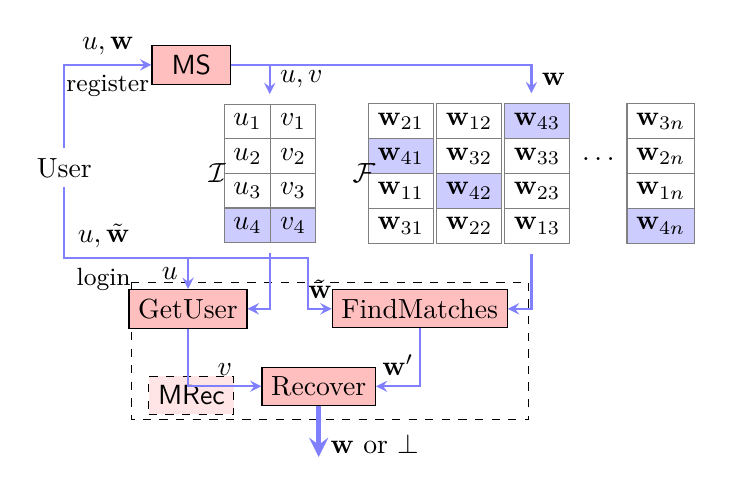
\begin{tikzpicture}[
    >=stealth,
    node distance=2cm,
    database/.style={
      cylinder,
      cylinder uses custom fill,
      cylinder body fill=black!25!white,
      cylinder end fill=black!25!white,
      shape border rotate=90,
      aspect=0.25,
      minimum width=2em,
      minimum height=2em,
      draw
    },
    func/.style={
      rectangle,
      fill=red!25!white,
      minimum width=1cm,
      minimum height=1em,
      draw
    },
    cell/.style={
      rectangle,
      draw=black!50!white
    }
    ]
    \node (user) at (0, 0) {User};
    \node[func, right of=user, right=-1.1em, above=3em] (msketch) {$\MS$}; 
    \draw[below of=msketch, dashed, anchor=west] (.85,0.55) rectangle (5.9,-1.2); 
    \node[func, below of=msketch, anchor=east, below=1.95cm,fill=red!10!white,dashed] (mrecover) {$\MRec$};
    % \node[database, right of=user, anchor=south, above=1em, right=2cm] (db1) {$\dbid$};
    \matrix (db1) [right of=user, anchor=south, below=2pt, right=-0.1cm, 
    matrix of math nodes,
    column sep = -\pgflinewidth,
    row sep=-\pgflinewidth,
    column 1/.style={nodes={cell}}, 
    column 2/.style={nodes={cell}}, 
    anchor=west] {
      \u_1 & \sketchval_1\\
      \u_2 & \sketchval_2\\
      \u_3 & \sketchval_3\\
      |[draw,fill=blue!20]|\u_4 & |[draw,fill=blue!20]|\sketchval_4\\
    };
    \node[left of=db1, anchor=east,right=1.1cm] {$\dbid$};
    \matrix (db2) [right of=db1, left=25pt, matrix of math nodes,
    column sep = 2\pgflinewidth,
    row sep=-\pgflinewidth,
    column 1/.style={nodes={cell}},
    column 2/.style={nodes={cell}}, 
    column 3/.style={nodes={cell}}, 
    column 4/.style={nodes={cell}}, 
    column 5/.style={nodes={cell}}, 
    anchor=west] {
      \mvec_{21} &\mvec_{12} & |[draw,fill=blue!20]|\mvec_{43} &  & \mvec_{3\mlen} \\
      |[draw,fill=blue!20]|\mvec_{41} &\mvec_{32} & \mvec_{33} & |[draw=white]|\ldots & \mvec_{2\mlen} \\
      \mvec_{11} &|[draw,fill=blue!20]|\mvec_{42} & \mvec_{23} &  & \mvec_{1\mlen} \\
      \mvec_{31} &\mvec_{22} & \mvec_{13} & & |[draw,fill=blue!20]|\mvec_{4\mlen} \\
    };
    \node[left of=db2, left=-4pt] {$\dbmsg$};

    % \node[database,right of=db1] (db2) {$\dbmsg$};
    \node[func,below of=db1,anchor=north,above=8pt,left=8pt] (gu) {GetUser};
    \node[func,right of=gu,anchor=east,right=-5pt] (fm) {FindMatches};
    \node[func,below of=db1,anchor=east,below=2em,right=-3pt] (recover) {Recover};

    \draw[->,blue!50,thick] (user.north) |- node[black,near end,above]{$u, \mvec$} node[black,near end,below,font=\small]{register} 
    (msketch.west);
    \draw[->,blue!50,thick] (msketch) -| node[black,near end, left,right]{$u, \sketchval$} (db1);
    \draw[->,blue!50,thick] (msketch) -| node[black,near end, left,right]{$\mvec$} (db2);

    \draw[->,blue!50,thick] (user.south) |- ++(1,-0.9) node[black,near end,above]{$u, \mvectilde$} node[black,near end,below,font=\small]{login}   -| node[black,left,near end]{$u$}
    (gu.north);
    \draw[->,blue!50,thick] (user.south) |- ++(0,-0.9)  -- ++(3.1,0) |- node[black,near end, above]{$\mvectilde$}
    (fm.west);
    \draw[->,blue!50,thick] (db1.south) |- node[black,near end,above]{} (gu.east);
    \draw[->,blue!50,thick] (db2.south) |- node[black,near end,above]{} (fm.east);
    \draw[->,blue!50,thick] (gu.south) |- node[black,near end,above]{$\sketchval$} (recover.west);
    \draw[->,blue!50,thick] (fm.south) |- node[black,near end,above]{$\mvec'$} (recover.east);    
    \draw[->,blue!50,line width=2pt] (recover.south) -- node[black,near end,right]{$\mvec$ or $\bot$} ++(0, -0.65);
  \end{tikzpicture}
  % \rcnote{Rough sketch of the flow of the \biosketch.} 
  \caption{Diagram of multisketch as a part of an authentication service. 
  }
  \label{fig:mainflow}
\end{figure}

%%% Local Variables:
%%% mode: latex
%%% TeX-master: "../main"
%%% End:


You refer to a figure in the following way. In~\figref{fig:mainflow} we show
some thing that is relevant for the Multisketch paper by Chatterjee et
al.~\cite{chatterjee2019multisketches}. Add your bibliography to the
\textsf{bib.bib} file. You can copy the Bibtex format citation from Google
Scholar.

\section{Tools and Methods}
\begin{itemize}
    \item \textbf{Device:} Samsung Galaxy S23 Ultra smartphone, running Android 15, equipped with the Snapdragon 8 Gen 2 Qualcomm SM8550-AB chipset, which supports dual-frequency, multi-constellation GNSS (GPS, Glonass, NavIC, Beidou, Galileo, QZSS). \cite{samsungs23ultra}
    \item \textbf{GNSS data collection:} "GNSSLogger" app, version 3.1.0.4 \cite{gnssLoggerApp} | "GPSTest" app, version 3.10.5 \cite{gpsTestApp} | "Google Earth" app, version 10.79.0.3. \cite{googleEarthApp}
    \item \textbf{Geoid height calculator:} GeographicLib web app. \cite{geoidHeightCalculator}
    \item \textbf{Data analysis:} MATLAB R2024b \cite{matlab} | gps-measurement-tools suite \cite{gpsMeasurementToolsCodebase}, developed by Google, enhanced by the NavSAS research group of Polytechnic of Turin \cite{navSAS} | "Location Based Analysis of Visible GPS Satellites" example notebook from MATLAB Satellite Communications Toolbox. \cite{skyplotsNotebook}
\end{itemize}
Every log contains 5 minutes of uninterrupted data sampled at [45.047208 N, 7.655716 W, 250 m a.s.l.] (Parco Cavalieri di Vittorio Veneto, Turin, Italy) (fig. \ref{fig:map}), isolated approximately 20 meters from nearby obstructions and under fair weather conditions, ensuring minimal multipath interference and optimal
reception. All user-space power-saving options were turned off and the device was put in Airplane mode during logging.
\label{sec:tools}

%%%%%%%%%%%%%%%%%%%%%%%%%%%%%%%%%%%%%%%%%%%%%%%%%%%%%%%%%%%%%%%%%%%%%%%%%%%%%%%%
\section{Scenario 1: Both Hosts on Ethernet}
\label{sec:wifi_water}
\begin{figure}[H]
    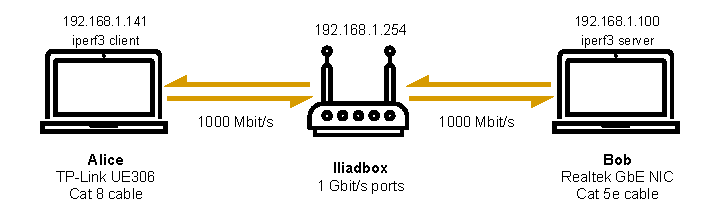
\includegraphics[width=0.90\linewidth]{images/wifi.drawio-4.pdf}
    \caption{Ethernet scenario}
    \label{fig:eth_to_eth_pic}
\end{figure}

\subsection{Scenario description}
For our first scenario, we set up the simplest network configuration: two hosts connected via Ethernet cables to the IliadBox router, which acted as a switch. Although this setup is straightforward, it is rarely used in everyday domestic environments. However, it remains widely prevalent in enterprise and corporate settings.

In this scenario, we had: Alice (\texttt{iperf3} client), IP: 192.168.1.141; Bob (\texttt{iperf3} server) with IP: 192.168.1.100.

\subsection{Computing the TMG}
In our setup, every device, adapter and port supports a maximum capacity of 1 Gbit/s. Therefore, we can assume the theoretical network capacity as $C = 1$ Gbit/s.

As discussed previously, when using an Ethernet connection in full-duplex mode, we need to account for the efficiency introduced by the various layers, namely Ethernet, IP and the transport layer protocol. We employed TCP, therefore, based on the previous theoretical computations (\ref{subsec:computations}), the TMG can be estimated as:
$$
\text{TMG} = \eta_{\text{TCPoFD}} \cdot C = 0.94 \cdot 1 \ \text{Gbit/s} = 940 \ \text{Mbit/s}
$$
This result reflects the expected goodput under ideal conditions, assuming no packet loss, latency, or other external disturbances. 
\subsection{Test results evaluation}
\begin{table}[htbp]
    \centering
    \caption{TCP Goodput from \texttt{iperf3} test (Mbit/s)}
    \label{tab:tcp-throughput-wired}
    \begin{tabular}{lrrrrc}
        \hline
        \textbf{Reverse flag} & \textbf{Avg} & \textbf{Median} & \textbf{Min} & \textbf{Max} & \textbf{Std Dev} \\
        \hline
        False & 937.6 & 938.0 & 937.0 & 938.0 & 0.49 \\
        True & 897.0 & 897.0 & 897.0 & 897.0 & 0.0 \\
        \hline
    \end{tabular}
    \end{table}

Table \ref{tab:tcp-throughput-wired} summarizes the \texttt{iperf3} test results for standard and reverse transmission modes.

In standard mode (reverse = False), the average goodput is 937.6 Mbit/s, with a median of 938.0 Mbit/s. The minimum (937.0 Mbit/s) and maximum (938.0 Mbit/s) values are close, resulting in a low standard deviation (0.49 Mbit/s), indicating stable performance. In reverse mode (reverse = True), the goodput remains constant at 897.0 Mbit/s, with zero variance, showing slightly lower yet stable performance. This difference may stem from transmission directionality or hardware handling.

Both configurations performed efficiently, with results close to the theoretical maximum goodput (950 Mbit/s).

By analyzing one of the PCAP files captured by the Python script, we can observe the overall behavior of the Ethernet scenario.

\begin{figure}[H]
    \centering
    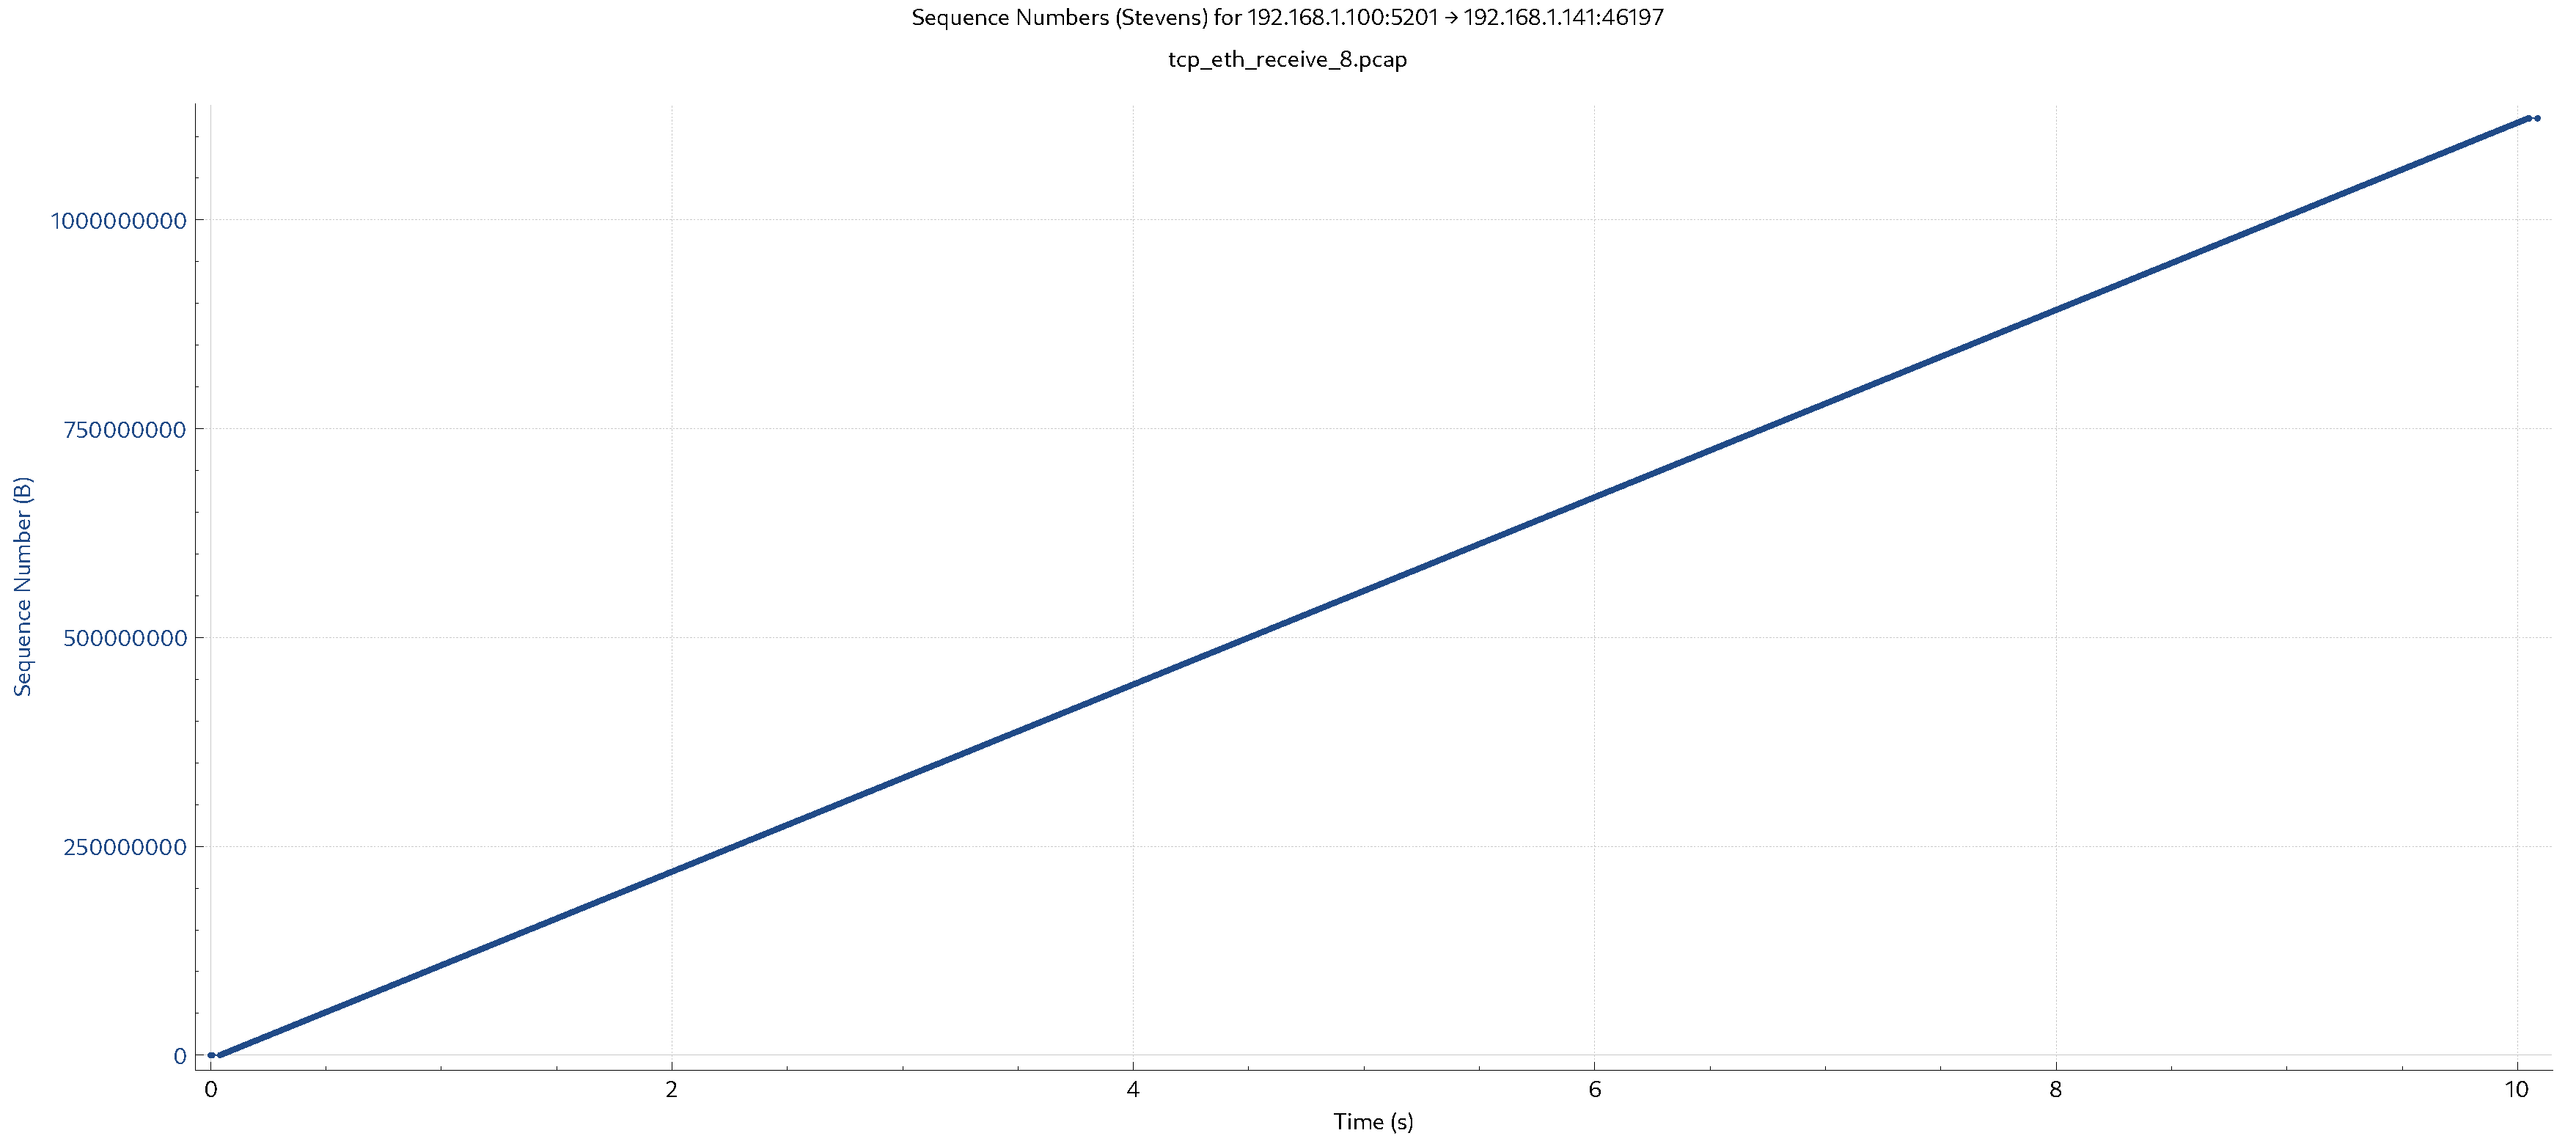
\includegraphics[width=0.75\linewidth]{SeqNumberEth.pdf}
    \caption{Sequence Numbers (Stevens), reverse flag set to True}
    \label{fig:enter-label}
\end{figure}


Looking at the graph that represents the sequence numbers of packets sent from the server (192.168.1.100) to the client (192.168.1.141) - which are the packets received when the reverse flag is enabled in \texttt{iperf3} - we notice that the graph forms a straight line. This indicates that the transmission occurred smoothly, without any retransmissions, and that the throughput remained consistent throughout the test.
We also plotted goodput computed by Wireshark.
\begin{figure}[H]
    \centering
    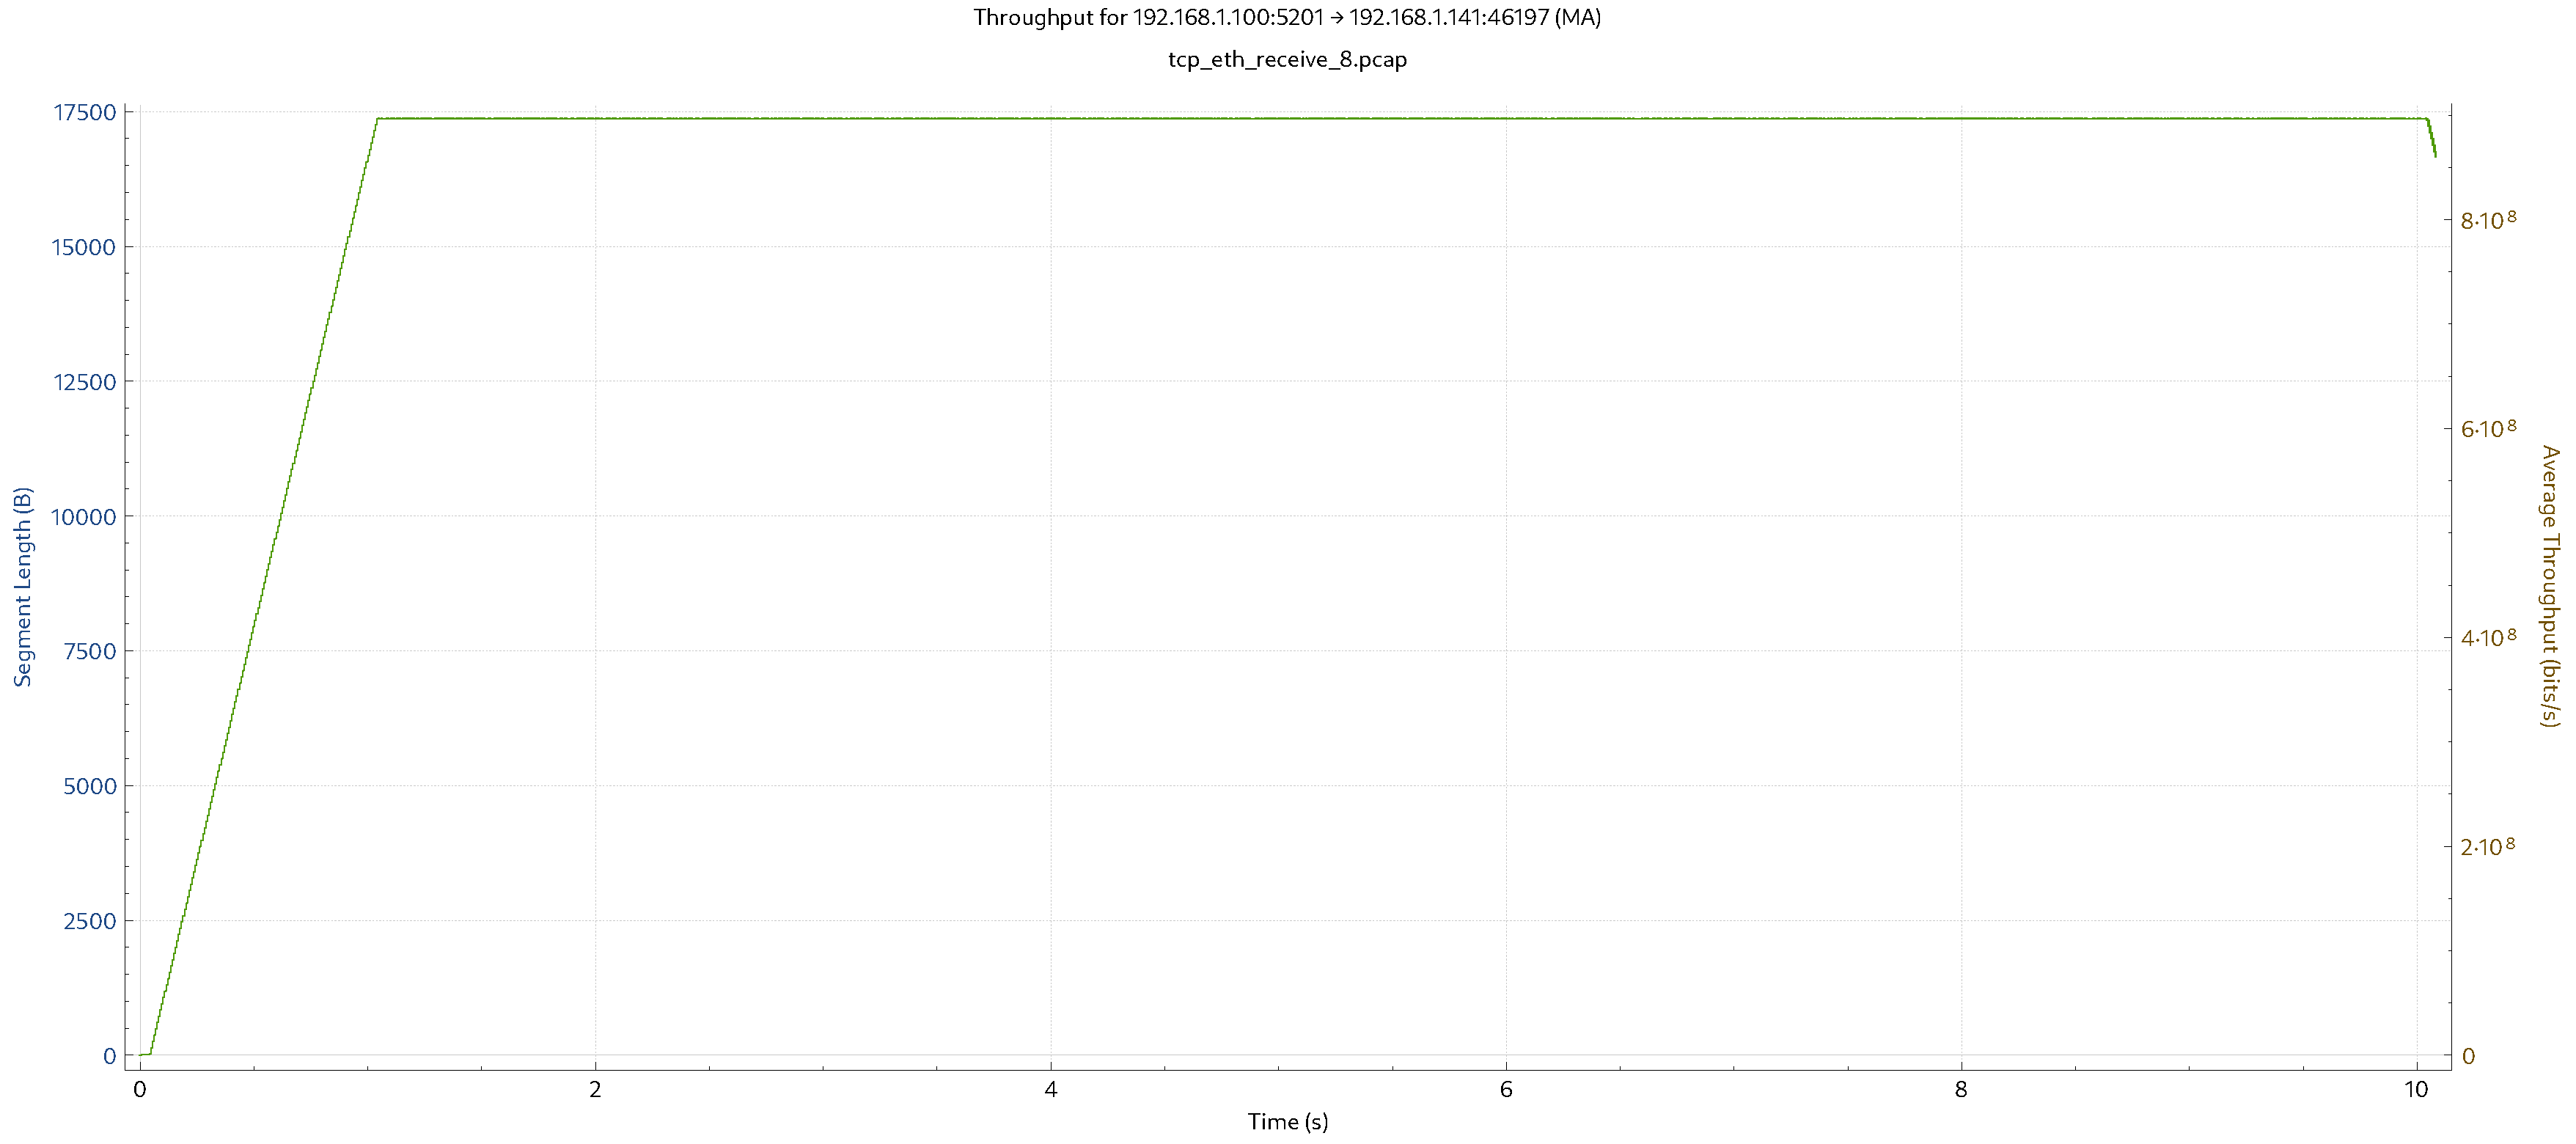
\includegraphics[width=0.75\linewidth]{GoodputEth.pdf}
    \caption{Goodput (MA) on the receiver side, reverse flag set to True}
    \label{fig:enter-label}
\end{figure}
It is important to note that we selected the "Goodput" option when generating the graph instead of "Throughput." 

However, we are unsure if Wireshark correctly differentiates between the two because both graphs appear identical.

%%%%%%%%%%%%%%%%%%%%%%%%%%%%%%%%%%%%%%%%%%%%%%%%%%%%%%%%%%%%%%%%%%%%%%%%%%%%%%%%
\section{SCENARIO 2: Both Hosts on Wi-Fi}
\label{sec:wifi}
\begin{figure}[h]
    \centering
    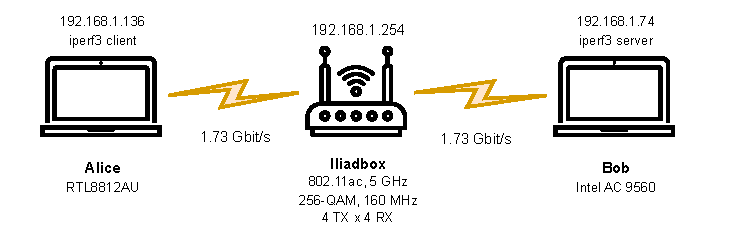
\includegraphics[width=0.95\linewidth]{images/wifi.drawio-3.pdf}
    \caption{Wi-Fi scenario}
    \label{fig:enter-label}
\end{figure}
\subsection{Scenario description}
For our second test, we benchmarked our LAN in the scenario of two hosts connected via Wi-Fi to the AP, far more common in the daily use of our home networks.

Using the same laptops as in the Ethernet test, now with Wi-Fi adapters, we configured the AP (same router as before) to enforce 802.11ac via the admin panel, from which we also confirmed it operated with 160 MHz channel bandwidth (eight 20 MHz channels combined) \cite{wikipedia_channelbonding} and 256-QAM modulation (combining amplitude and phase shifts to encode 8 bits in a symbol) \cite{wikipedia_qam}.

In this scenario, we had: Alice (\texttt{iperf3} client), IP: 192.168.1.136; Bob (\texttt{iperf3} server) with IP: 192.168.1.74.

\subsection{Computing the TMG}
Based on our information and on the router specifications (in particular, the number of antennas, which is 4 TX x 4 RX for the 5 GHz band), it has been easy to know about the capacity $C$ of the physical link in such a configuration \cite{wikipedia_80211ac}.
We have in fact a nominal capacity $C=1.73$ Gbit/s for both physical links, since both the clients are equipped with 2 TX x 2 RX antennas and support MU-MIMO. 

These numbers are to some degree confirmed by the statistics computed by the OS of our devices.
The TMG for the communication has been estimated using the equation:
\begin{align*}
    \text{TMG}&=\eta_{\text{TCPoHD}}\cdot\eta_{\text{802.11}}\cdot (0.5\cdot C)\\&=0.89\cdot 0.80\cdot (0.5\cdot1.73\text{ GBit/s)}=616\text{ Mbit/s}
\end{align*}
which takes into account the fact that every frame has to be transmitted twice (hence the factor 0.5), once from the sender to the AP and then from the AP to the recipient.
From the equations, TMG is 616 Mbit/s. We expect this to be valid for both directions ($A\to B$ and $B\to A$).

\subsection{Test results evaluation}
\begin{table}[htbp]
    \centering
    \caption{TCP Goodput from \texttt{iperf3} test (Mbps)}
    \label{tab:TCPoHD-throughput}
    \begin{tabular}{lrrrrc}
        \hline
        \textbf{Reverse flag} & \textbf{Avg} & \textbf{Median} & \textbf{Min} & \textbf{Max} & \textbf{Std Dev} \\
        \hline
        False & 192.0 & 193.5 & 177.0 & 197.0 & 5.42 \\
        True & 147.3 & 147.0 & 143.0 & 150.0 & 2.00 \\
        \hline
    \end{tabular}
\end{table}

The test results clash with our expectations; in fact, we have a third of the \text{TMG} in the direction $A\to B$ and even a lower goodput for the direction $B\to A$. 
We dived deeper in the specifications of all the devices, discovering that the RTL8812AU chipset is only capable of exploiting channel bandwidths up to 80 MHz. Our estimation needs now to take into account the disparity in the speeds of the two links, with the ${A\leftrightarrow AP}$ link being the bottleneck. In particular, the overall capacity is not anymore $0.5\cdot C$, since the two channels have different transmission speeds:
\begin{itemize}
    \item $C_{A\leftrightarrow AP}= C/2 = 867$ Mbit/s
    \item $C_{B\leftrightarrow AP}= C = 1.73$ Gbit/s
\end{itemize}
% \begin{equation}
% \begin{cases}
%     T_{\text{data, C1}}&=\frac{\sub{MSS}{TCPoHD}}{\sub{TMG}{802.11, C1}}=\frac{1460\ \text{B}}{867\ \text{Mbit/s}}=13.5\ \si{\micro\second}\\
%     T_{\text{overhead, C1}}&=\frac{\sub{Header}{TCPoHD}+\sub{Header}{IP}+\sub{Overhead}{Eth}}{\sub{TMG}{802.11, C1}}\\&=\frac{20+20+38\ \text{B}}{867\ \text{Mbit/s}}=0.72\ \si{\micro\second}\\
%     T_{\text{data, C2}}&=\frac{\sub{MSS}{TCPoHD}}{\sub{TMG}{802.11, C2}}=\frac{1460\ \text{B}}{1.73\ \text{Gbit/s}}=6.75\ \si{\micro\second}\\
%     T_{\text{overhead, C2}}&=\frac{\sub{Header}{TCPoHD}+\sub{Header}{IP}+\sub{Overhead}{Eth}}{\sub{TMG}{802.11, C1}}\\&=\frac{20+20+38\ \text{B}}{1.73\ \text{Gbit/s}}=0.36\ \si{\micro\second}\\
%     \eta_\text{links}&=\frac{T_{\text{data, C2}}}{T_{\text{data, C1}} + T_{\text{data, C2}} + T_{\text{overhead, C1}} + T_{\text{overhead, C2}}}=32\%\\
%     G&= \eta_\text{links}
% \cdot\eta_{\text{TCPoHD}}\cdot\eta_{\text{802.11}}\cdotC_{\text{802.11},\ A\leftrightarrow AP}}
% \end{cases}
% \end{equation}
Let $C'$ be the new overall capacity. Then:
\begin{equation*}
\begin{cases}
    C'&=\frac{\text{Data}}{\text{TX Time}}=\frac{\text{Data}}{\text{TX Time }(A\leftrightarrow AP)\ +\ \text{TX Time }(AP\leftrightarrow B)}
    \\&=\frac{\text{Data}}{\frac{\text{Data}}{C_{A\leftrightarrow AP}}+\frac{\text{Data}}{C_{B\leftrightarrow AP}}}
    \\&=\frac{1}{1/C_{A\leftrightarrow AP}\ +\ 1/C_{B\leftrightarrow AP}}=\frac{1}{3}\cdot C=578\text{ Mbit/s}\\
    \text{TMG}&= \eta_{\text{TCPoHD}}\cdot\eta_{\text{802.11}}\cdot C'\\&=0.89\cdot0.80\cdot578\text{ Mbit/s}=411\text{ Mbit/s}
\end{cases}
\end{equation*}
The new equations estimate a TMG of 411 Mbit/s, but discrepancies from the results persist, likely due to signal attenuation, interference from neighbour networks, and unknown device limitations. 

Similar to Ethernet, we also have to tackle the loss of goodput (-23\%) when communicating in the $B\to A$ direction with respect to the $A\to B$ direction. We are unsure on what caused the discrepancy, which is nonetheless consistent across several tests. While the reciprocity principle \cite{balanis2005antenna} suggests symmetrical TX/RX performance, real antennas include additional components that may introduce asymmetries.
We hypothesize that 802.11ac optimizes the downlink, as switching to 802.11n @ 2.4 GHz reversed the effect. No other configuration adjustments (client-server swap, device variation, UDP use) made the trend change.

As seen in the Ethernet scenario, we now examine the sequence number and goodput graphs for this case as well. In this PCAP instance, we observe that no retransmissions occurred. 
\begin{figure}[H]
    \centering
    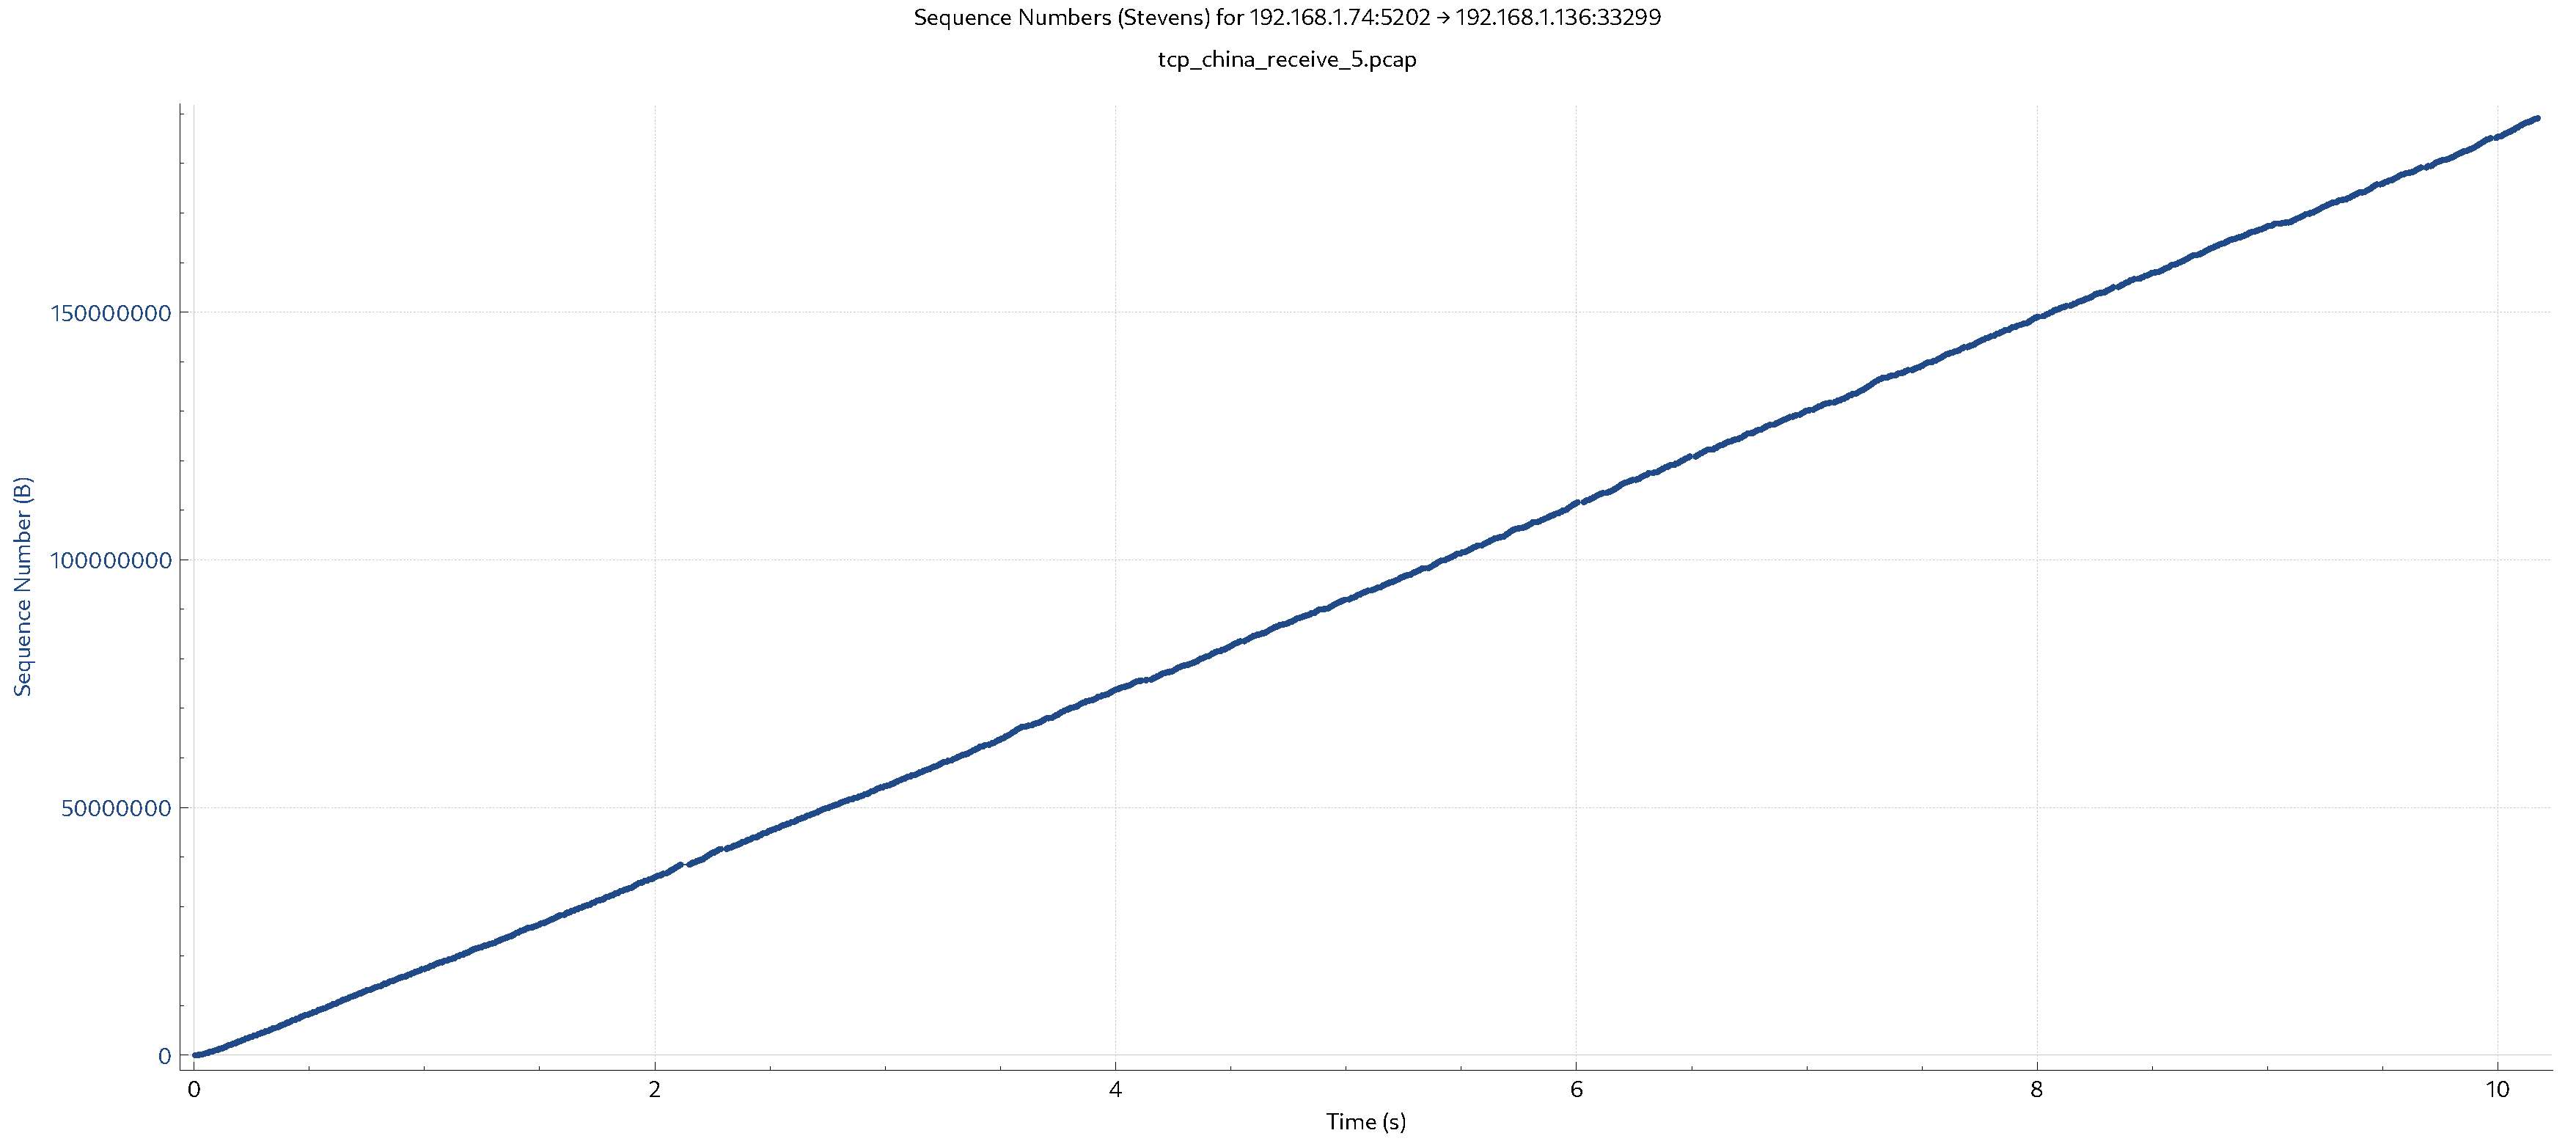
\includegraphics[width=0.75\linewidth]{images/SeqNumberChina.pdf}
    \caption{Sequence Numbers (Stevens), reverse flag set to True}
    \label{fig:enter-label}
\end{figure}

However, unlike the Ethernet scenario, the goodput shows more fluctuation over time (it is no longer a flat, horizontal line but displays small oscillations), indicating the presence of a less stable wireless channel. 

\begin{figure}[H]
    \centering
    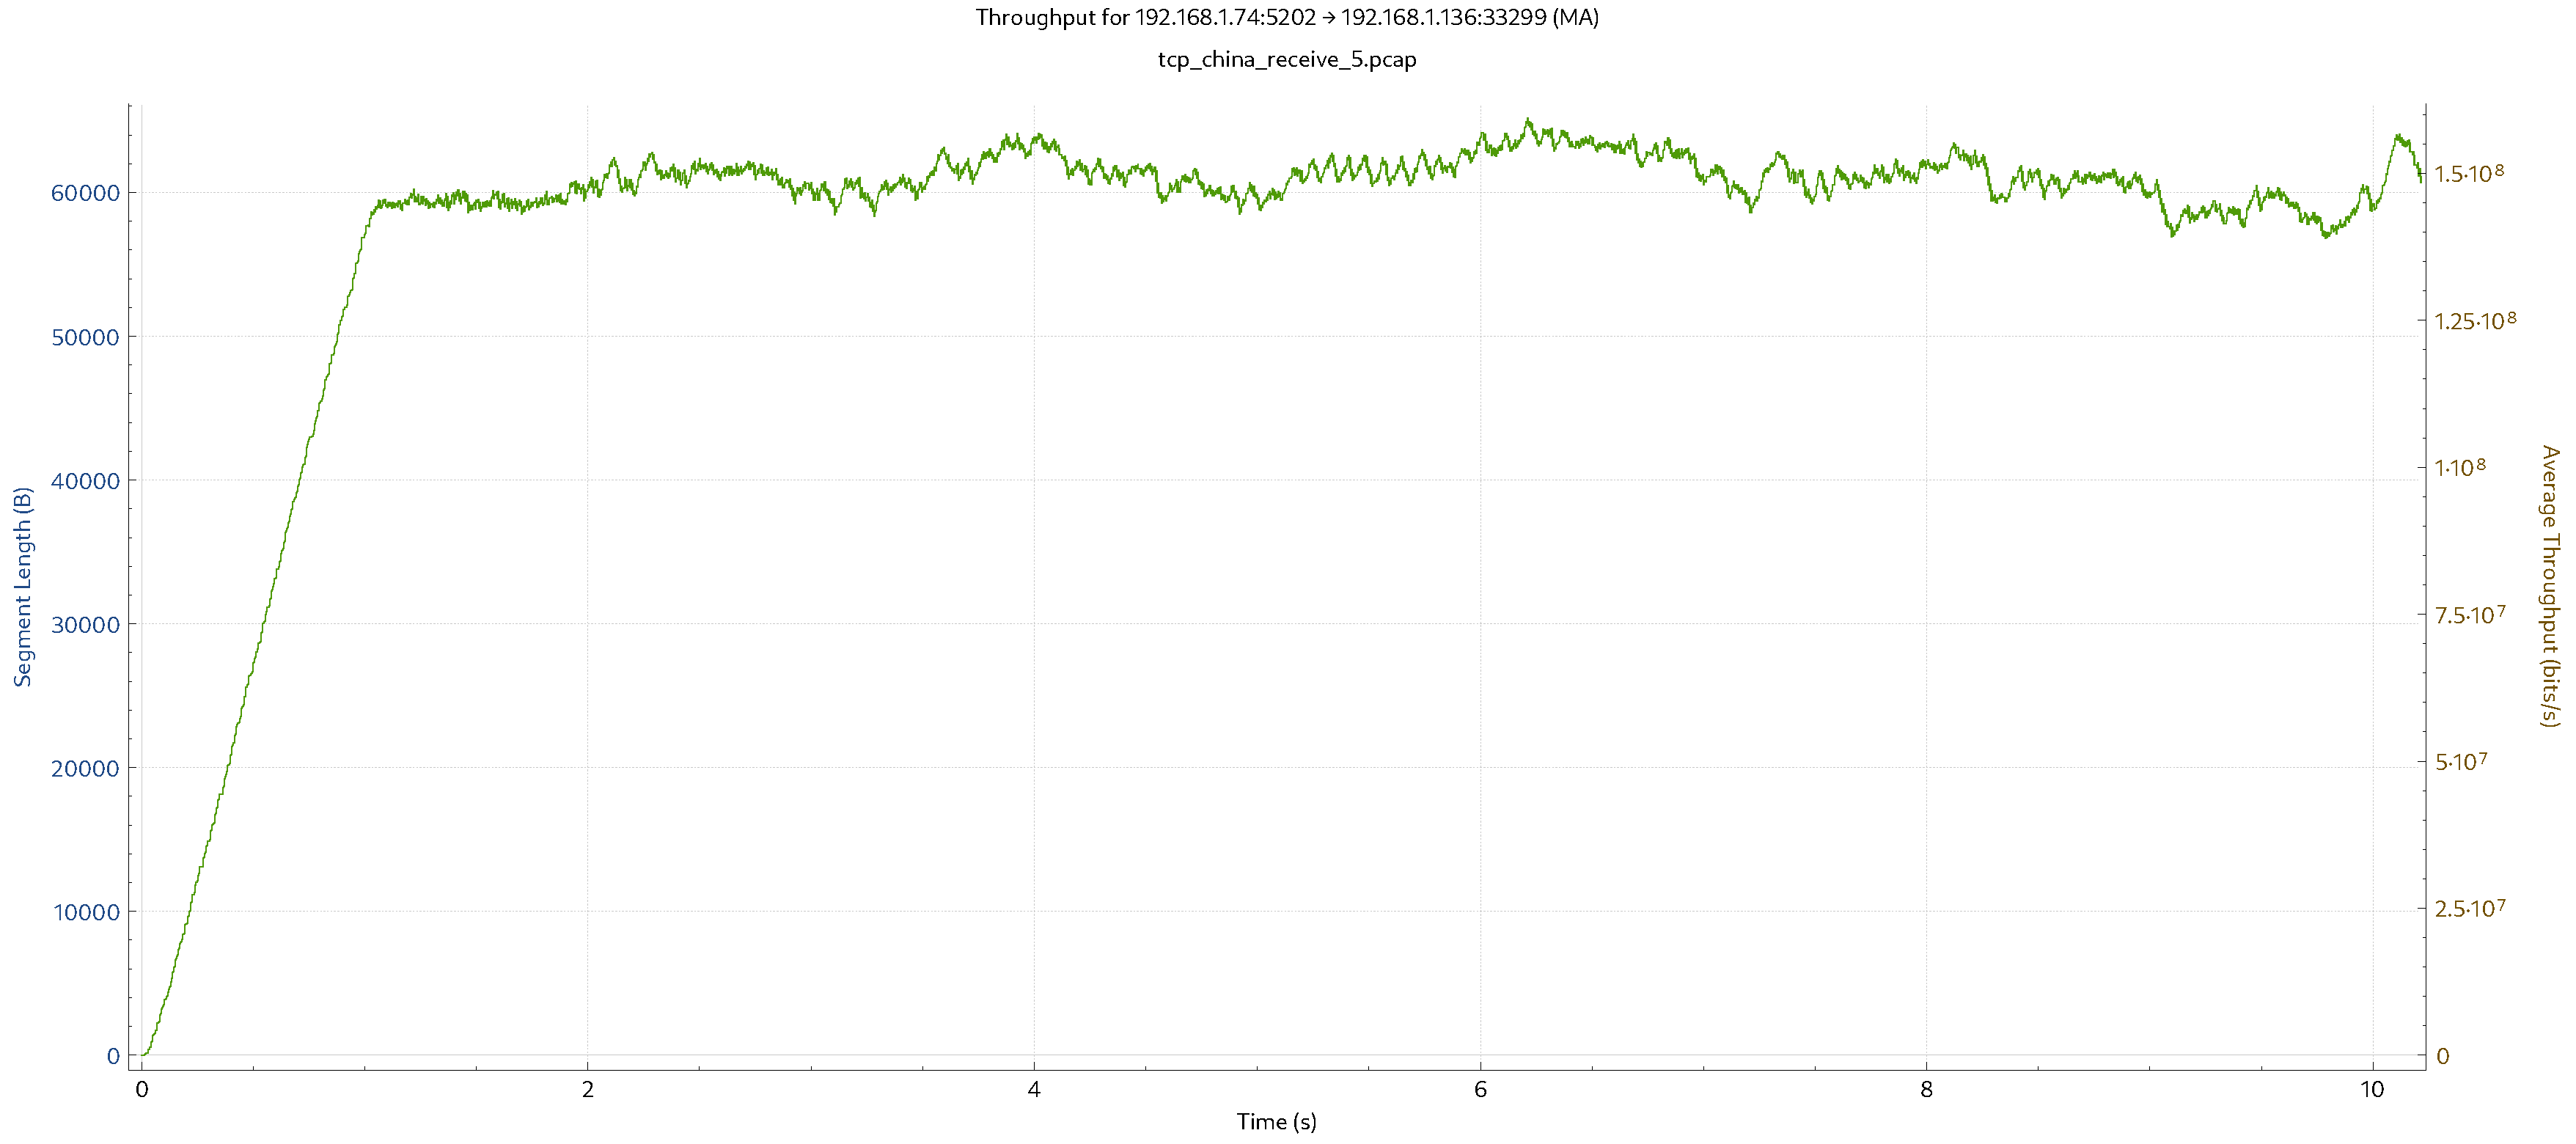
\includegraphics[width=0.75\linewidth]{images/GoodputChina.pdf}
    \caption{Goodput (MA) on the receiver side, reverse flag set to True}
    \label{fig:enter-label}
\end{figure}

The goodput is also significantly lower than in the Ethernet case.
The average goodput calculated from the different \texttt{iperf3} tests is 147.3 Mb/s, which closely matches the value observed on Wireshark (above 150 Mb/s, as shown in the graph). The slight discrepancy can be attributed to the seventh test, which performed worse than the others (with retransmissions observed), causing a drop in the overall average goodput.
%%%%%%%%%%%%%%%%%%%%%%%%%%%%%%%%%%%%%%%%%%%%%%%%%%%%%%%%%%%%%%%%%%%%%%%%%%%%%%%%
\section{Scenario 3: Both Hosts on Wi-Fi, one Submerged in Seawater}

\label{sec:wifi_water}
\begin{figure}[h]
    \centering
    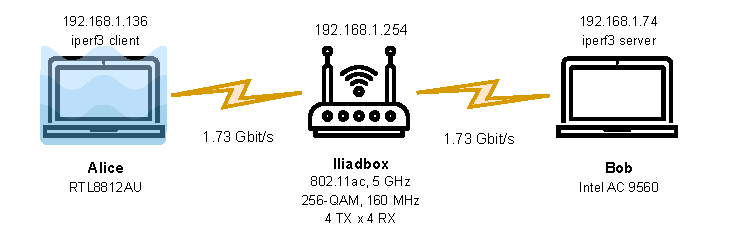
\includegraphics[width=0.95\linewidth]{images/wifi_water.drawio.pdf}
    \caption{Seawater scenario}
    \label{fig:wifi_to_wifi_water_pic}
\end{figure}

\subsection{Scenario description}
For our third test, we explore how Wi-Fi connections work underwater. This may happen in scenarios such as sensor analysis for water quality and oil spill detection, or submarine communications and mine detection and neutralization. We designed an experiment in which one Wi-Fi-connected host was submerged in seawater while the other host was not.
To replicate this, we enclosed the directional antenna in a waterproof silicone material. Subsequently, we submerged the antenna in 5 cm of water with a salt concentration of 35\%.

Our test setup consisted of the same two hosts with identical configurations in the previous scenario (\ref{sec:wifi}). The only variable introduced was the addition of water for the host equipped with the directional antenna.

\subsection{Consideration on the TMG}
The salinity of water significantly impacts electromagnetic (EM) wave propagation, leading to higher attenuation compared to free-space conditions. This is due to changes in the water's permittivity, which is influenced by the dipole moment of water molecules, and the increased conductivity resulting from the ionization of added salt. Pure water has low conductivity because its molecules are not naturally polarized, but the introduction of salt enhances conductivity, further increasing the EM wave attenuation.

Based on these factors, we expect a substantial reduction in throughput in saline water, primarily due to the high attenuation of EM waves. The increased conductivity and dielectric properties of seawater are likely to degrade signal quality and lower the data transfer rate. \cite{arrabitothesis}

In the previous experiment conducted in air, we observed a goodput of 192 Mbit/s under conventional conditions (\ref{sec:wifi}). However, when submerged in seawater, we anticipate that signal attenuation, potential multipath effects and wave absorption will significantly reduce goodput.


\subsection{Test results evaluation}


\begin{table}[H]
    \centering
    \caption{TCP Goodput from \texttt{iperf3} test (Mbps)}
    \label{tab:tcp-throughput-wifi}
    \begin{tabular}{lrrrrc}
        \hline
        \textbf{Reverse flag} & \textbf{Avg} & \textbf{Median} & \textbf{Min} & \textbf{Max} & \textbf{Std Dev} \\
        \hline
        False & 3.499 & 3.81 & 1.13 & 5.47 & 1.49 \\
        True & 9.914 & 9.985 & 5.86 & 14.6 & 2.72 \\
        \hline
    \end{tabular}
\end{table}
During the experiments we noted, observing the router's admin panel, how Alice's network card was hopping from one configuration to another. In particular, it autonomously downgraded its connection from the 5 GHz band to a slower standard in the 2.4 GHz band. In general, the results of this experiment align with our expectations regarding the impact of seawater on Wi-Fi performance. As discussed previously, the presence of saltwater significantly attenuates electromagnetic waves (EM), which in turn degrades the throughput and reliability of wireless networks. 

This scenario also reveals differences in signal performance between transmission and reception modes. Among the various reasons for this, we could consider the high unrealiability of the channel as the main cause. In fact, other technologies are often used for underwater communication. Acoustic waves, similar to sonar, are the most common method, as they travel efficiently through water and are used in submarines and underwater research (\ref{sec:underwater-comm}) \cite{arrabitothesis}.

Moving on to examine the sequence number graph for this scenario, we can immediately notice that the slope of the curve is less steep compared to previous scenarios. This suggests a lower overall throughput. 

\begin{figure}[H]
    \centering
    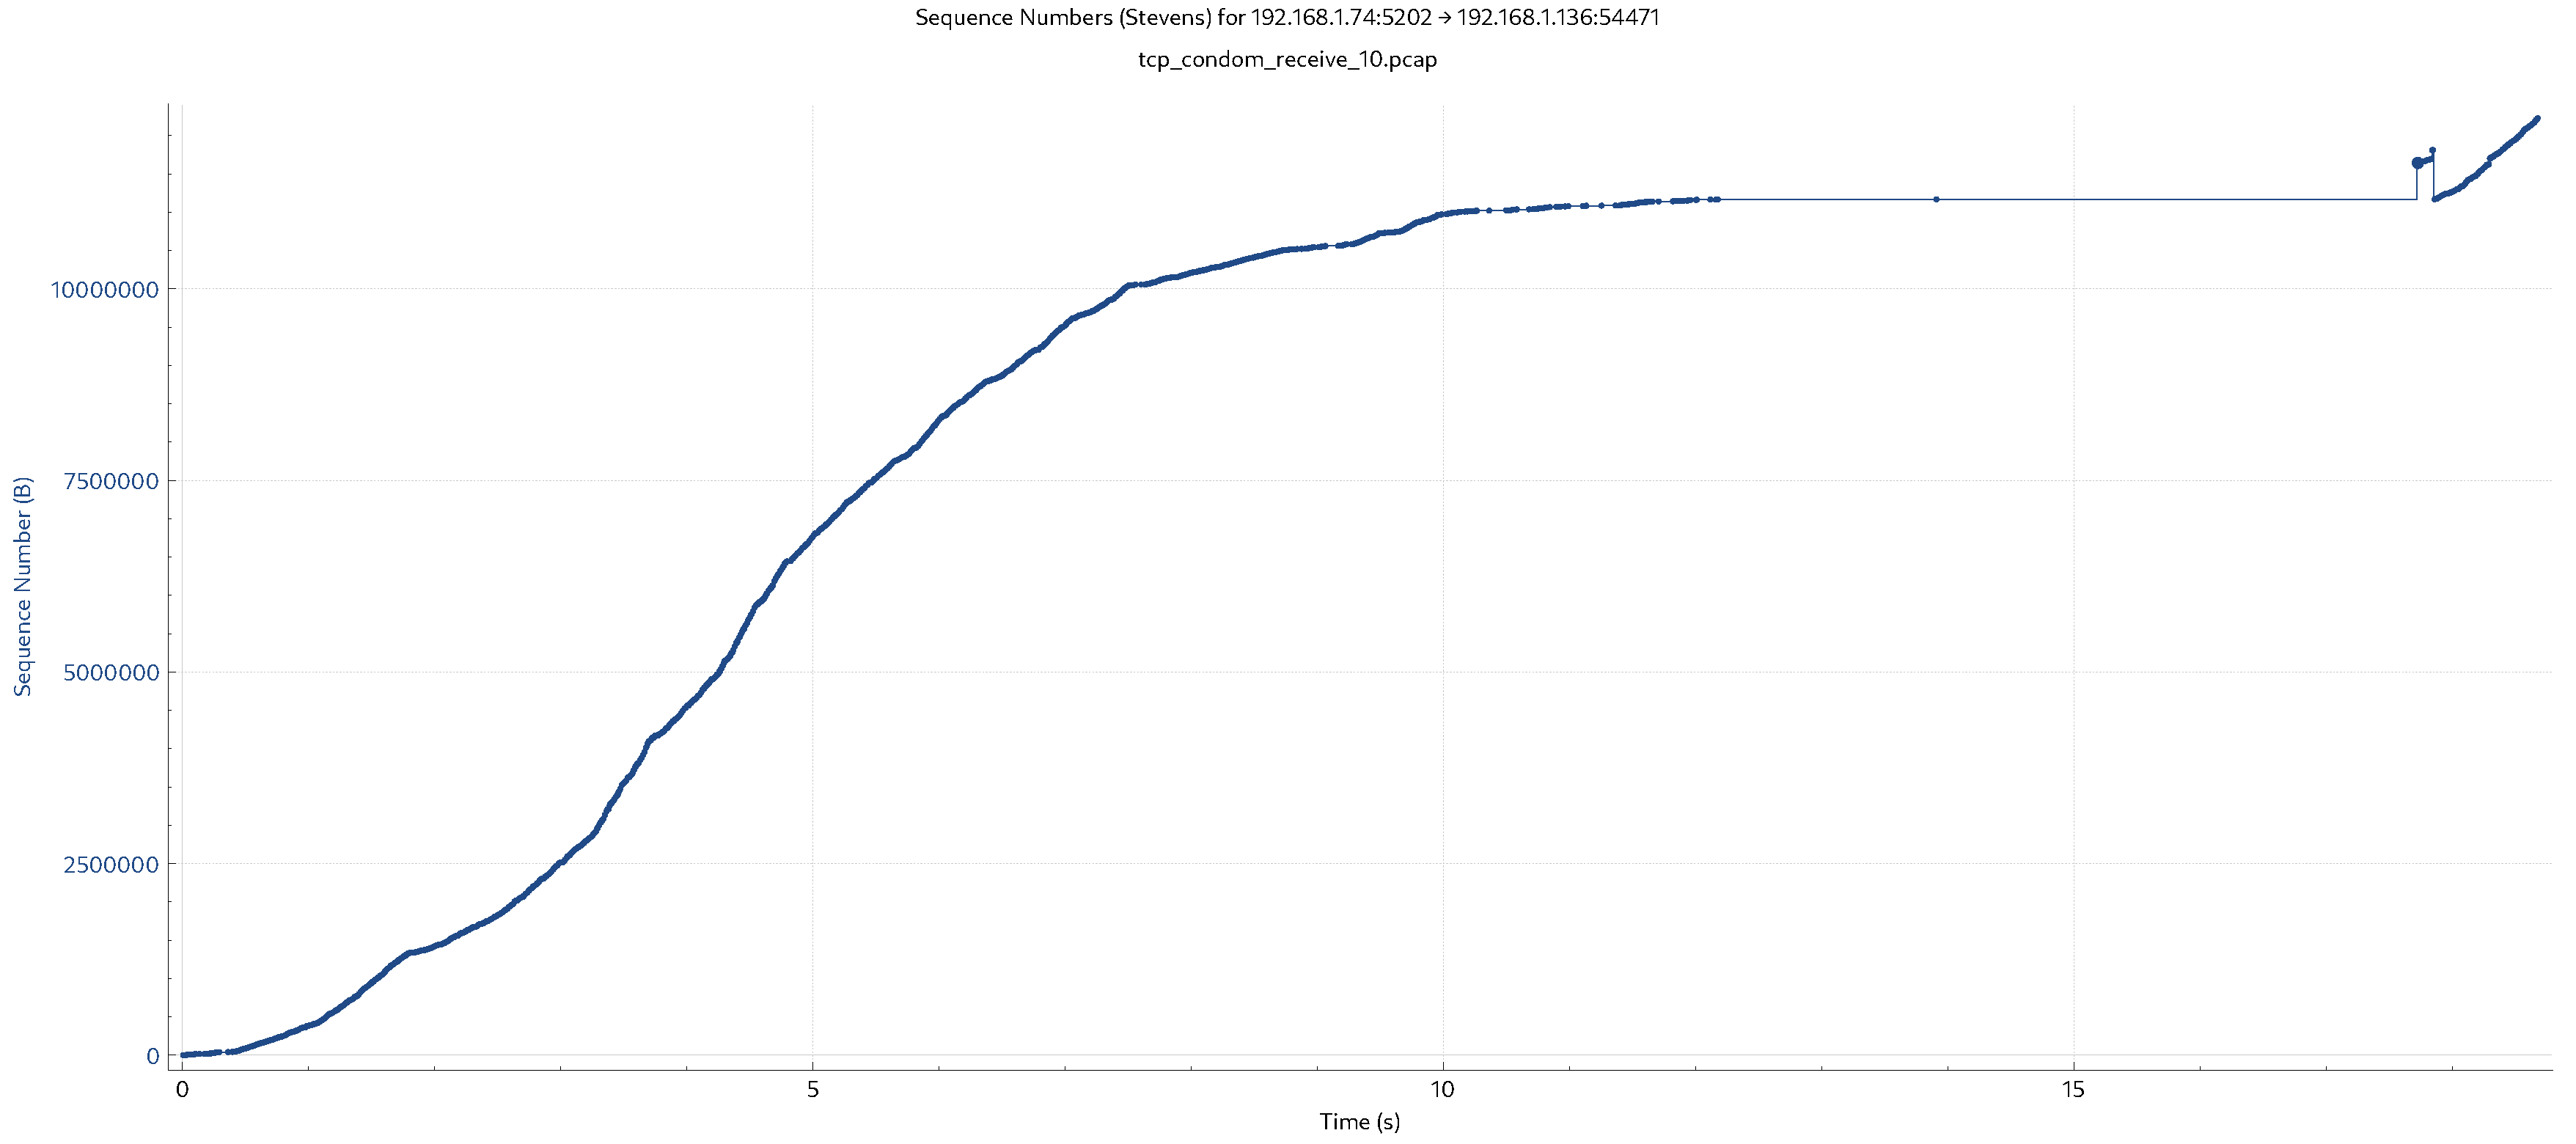
\includegraphics[width=0.75\linewidth]{images/SeqNumSaltWater.pdf}
    \caption{Sequence Numbers (Stevens), reverse flag set to True}
    \label{fig:enter-label}
\end{figure}

Additionally, the transmission lasted longer than the 10 seconds we set in the test parameters. 
This is evident from the graph, where towards the end of the transmission, the slope flattens (forming a horizontal line), indicating that no data was being received at that point. This is due to the need for retransmissions, as shown by the drop in the sequence number at one point. These retransmissions and the presence of duplicate ACKs are confirmed by using specific Wireshark filters and observing the TCP errors graph (\ref{graficoCiro}).

The second graph, which shows the outstanding bytes (bytes that have been sent but have not yet been acknowledged), further confirms that retransmissions occurred later in the transmission. This behavior can be better understood when examining the receiving window graph. The recWin shows how much data the receiver can accept at a given time. The recWin graph fluctuates continuously, suggesting that the system was adjusting dynamically due to network congestion or other factors. 

\begin{figure}[H]
    \centering
    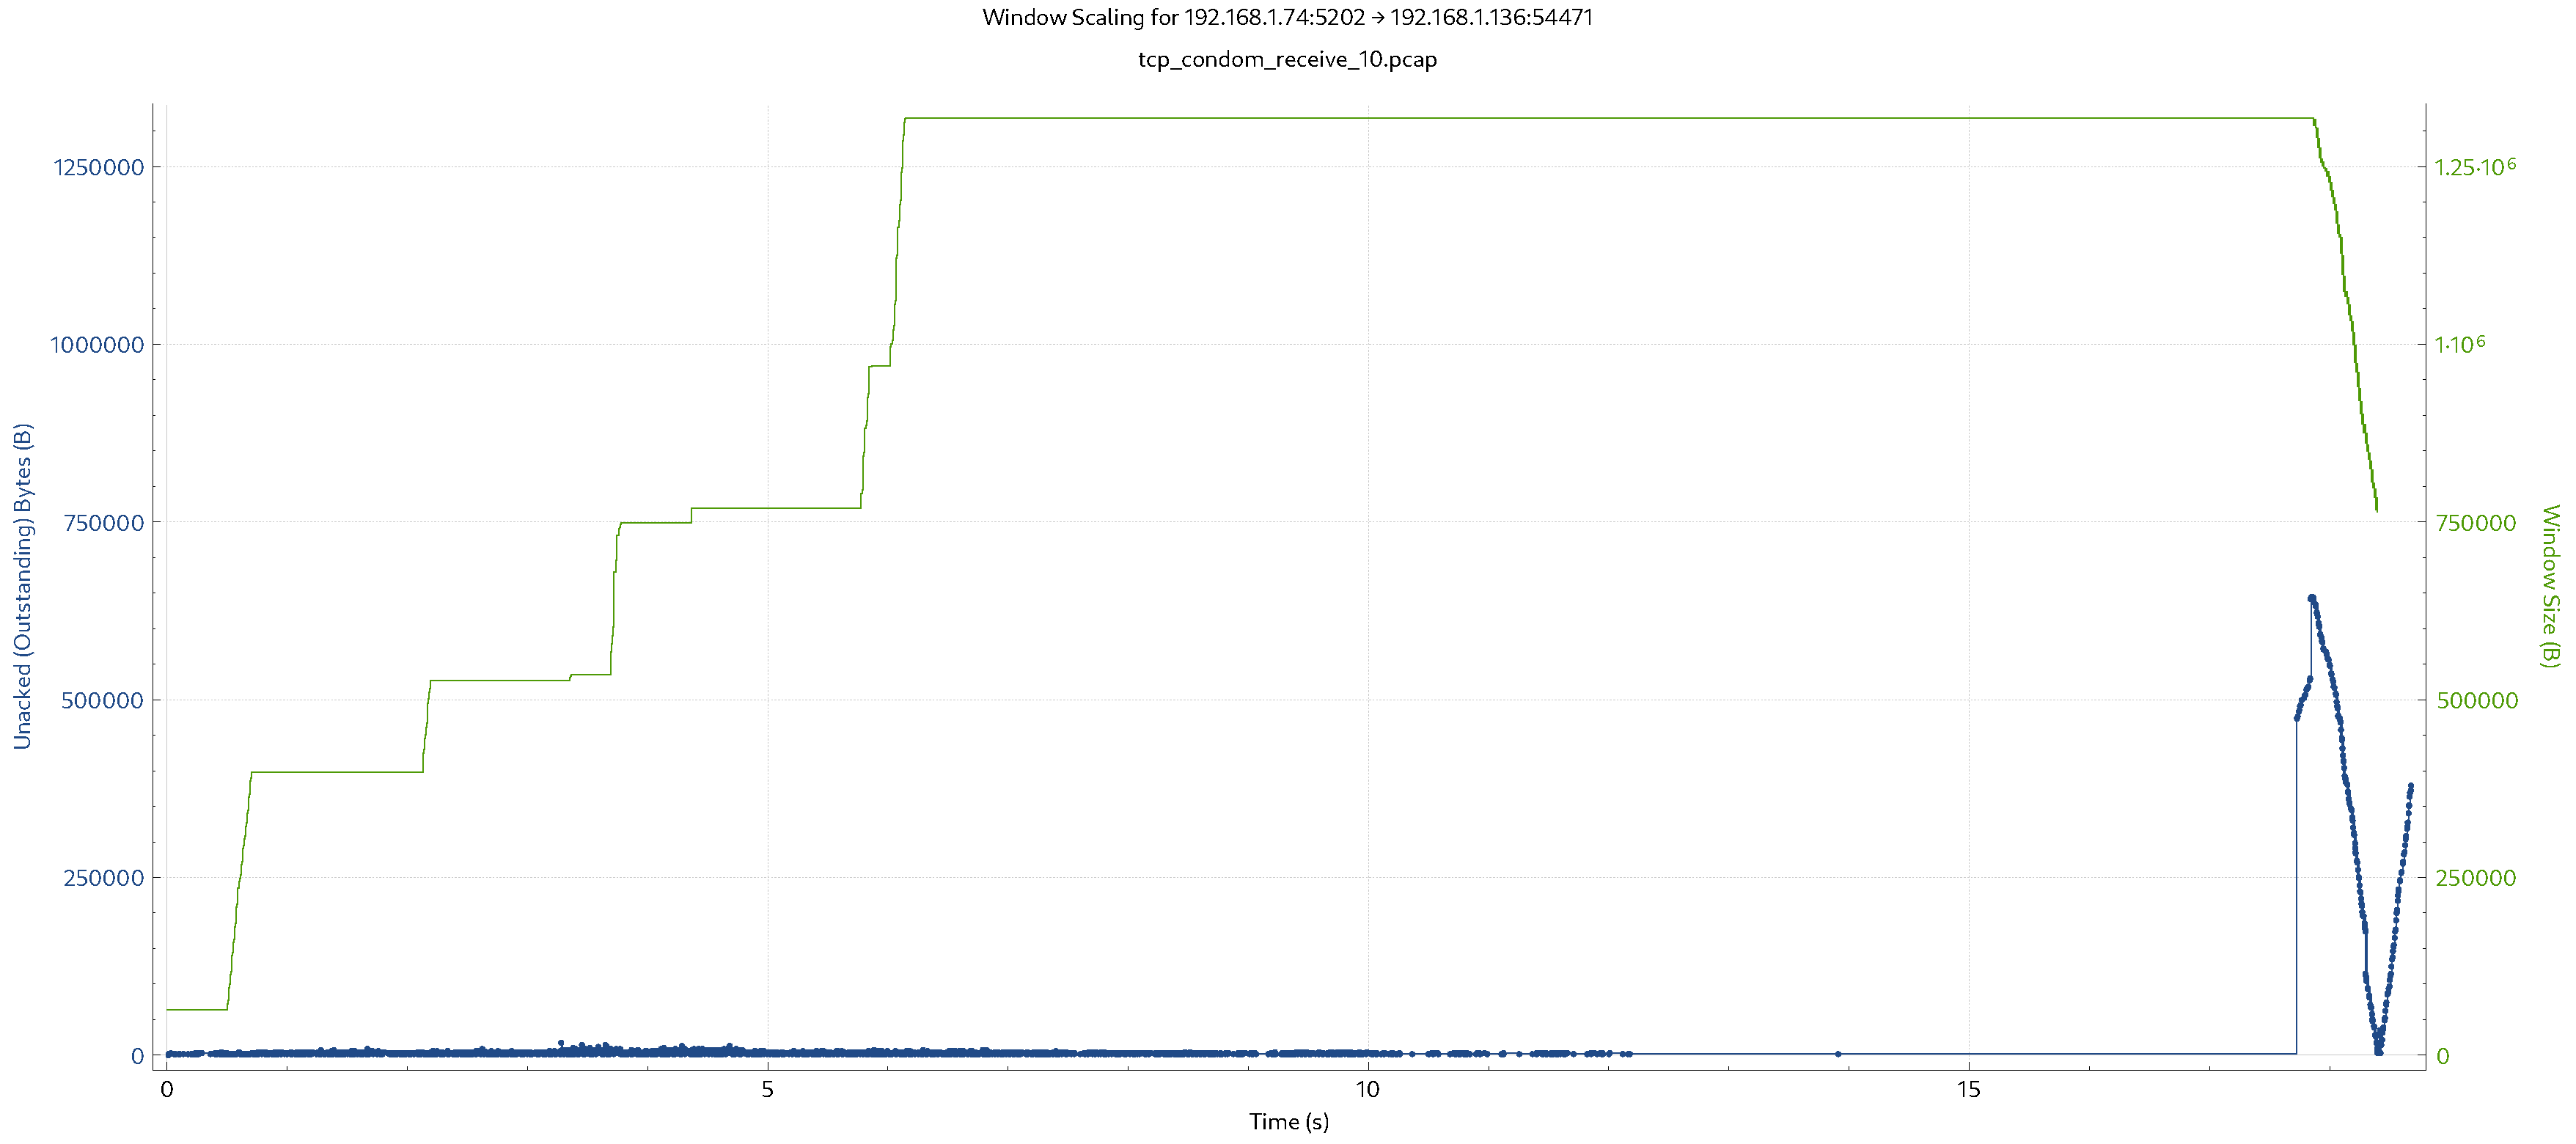
\includegraphics[width=0.75\linewidth]{RecWinSaltWater.pdf}
    \caption{OutBytes and recWin size on the client, reverse flag set to True}
    \label{fig:enter-label}
\end{figure}

Unlike other scenarios, where the recWin remains stable, the continuous change in this case indicates that the submerged receiver dynamically adjusted its window size, likely due to fluctuating network conditions during the test. This adjustment was a preventive measure to avoid overloading the receiver. In fact, if the receiver experiences high traffic or delays, it may reduce the window size to prevent overloading, causing fluctuations in the recWin even without the need for retransmission.

In conclusion, the experiment validated our initial predictions regarding the catastrophic impact of seawater on EM wave propagation.
\section{Conclusion}
\label{sec:conclusion}

% The analysis of the different scenarios clearly shows that wired network transmission maintains a high level of stability. The simplicity of the setup and the use of Ethernet cables allow for accurate theoretical estimations of goodput, as the variables involved are limited and controllable. At the same time, it is clear how this significantly changes when moving to wireless communication. The wide range of technologies and protocols available in 2025 makes it challenging to obtain precise theoretical estimates of goodput, and even after conducting additional analyses, computeing accurate predictions remains complex.  
% Finally, we observed how highly variable environments like saline water make empirical evaluations the only reliable approach.

% In conclusion, this study highlights the importance of considering transmission environment characteristics and device specifications to obtain realistic goodput estimations, especially for wireless and unconventional communication scenarios.

Despite our computations being somewhat approximative, we can still extract valuable insights.
Wired networks offer stable transmission, allowing accurate goodput estimations due to controlled variables. In contrast, wireless communication introduces complexity, making precise theoretical predictions challenging, because of the wide range of technologies of 2025. Finally, empirical evaluation remains essential, particularly in highly variable environments like saline water. 






\bibliographystyle{ACM-Reference-Format}
\bibliography{bib}

% % --- Appendix ---%
\appendix
\onecolumn
\section{Additional plots}
\label{sec:additional_plots}

\begin{figure}[H]
    \centering
    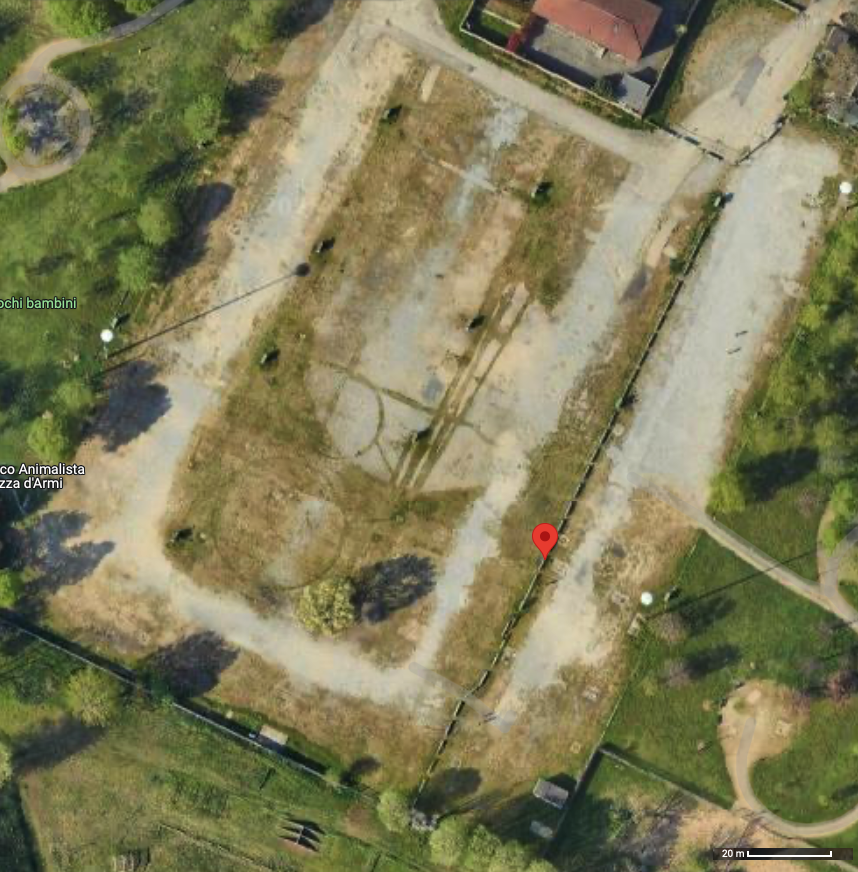
\includegraphics[width=0.5\linewidth]{images/map_place.png}
    \caption{Place where all surveys were carried out.}
    \label{fig:map}
\end{figure}

% \begin{figure}[H]
%     \centering
%     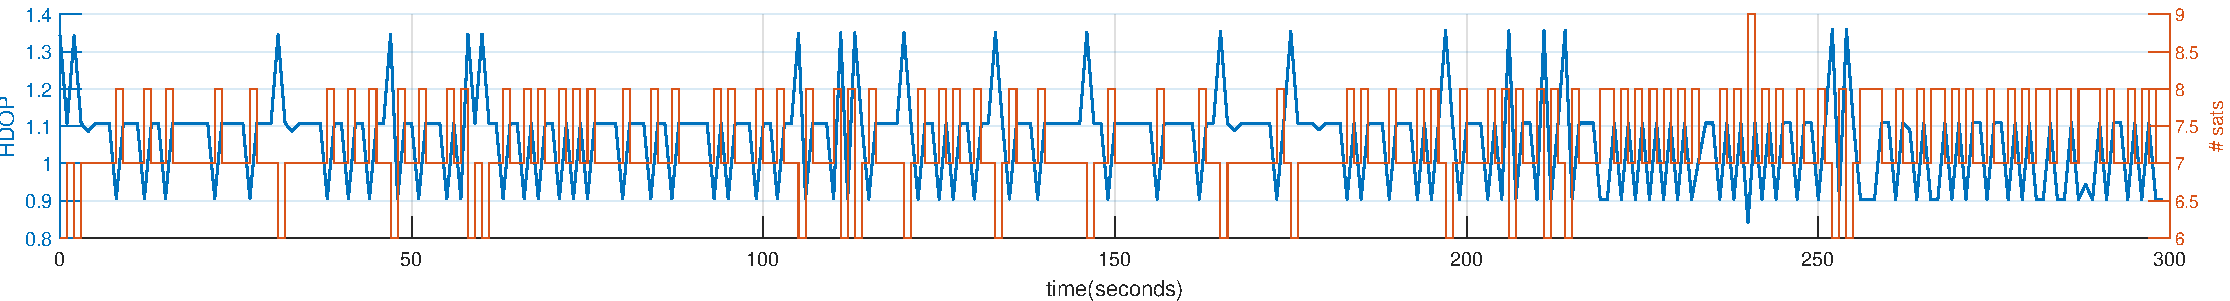
\includegraphics[width=1.00
%     \linewidth]{images/carne_hdop_carne.pdf}
%     \caption{HDOP and SATs number in the interference scenario}
%     \label{fig:carne_hdop}
% \end{figure}

\begin{figure}[H]
    \centering
    \begin{minipage}[b]{0.48\linewidth}
        \centering
        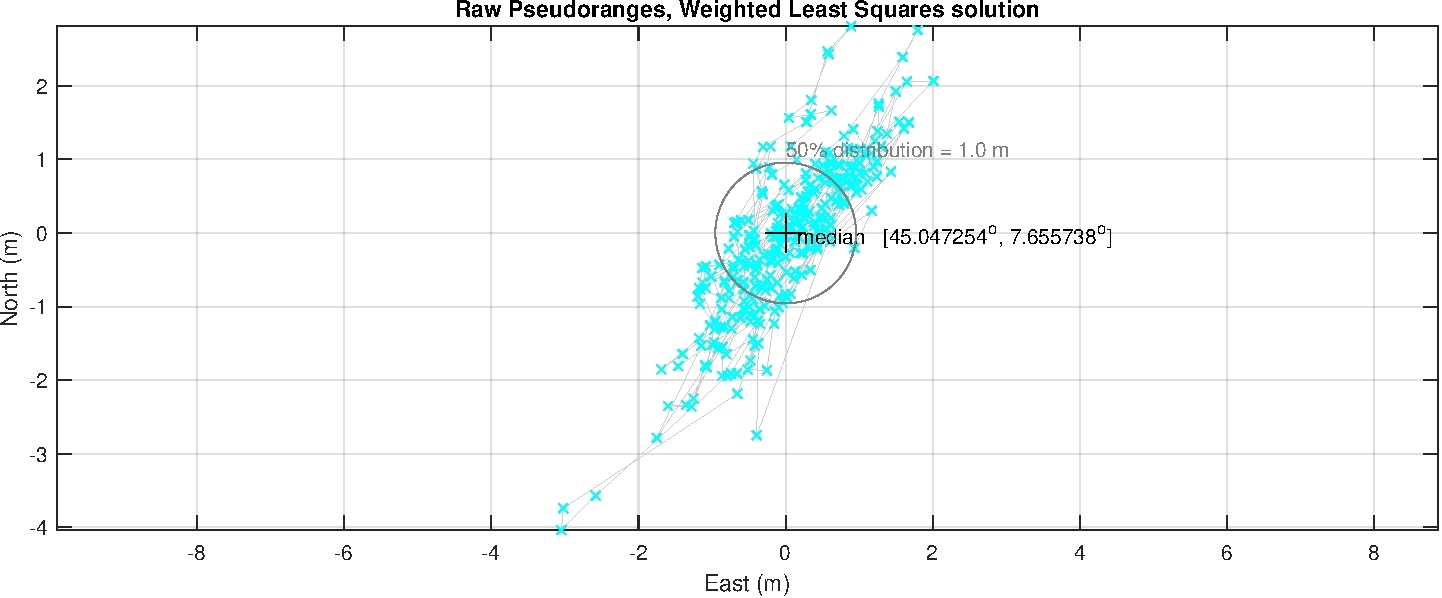
\includegraphics[width=1.00\linewidth]{images/pos_punto_3_precision.pdf}
        \caption{Positioning geoplot for logs collected in open-sky conditions (\ref{sec:opensky})}
        \label{fig:pos_punto_3_precision}
        \end{minipage}
    \hfill
    \begin{minipage}[b]{0.48\linewidth}
        \centering
        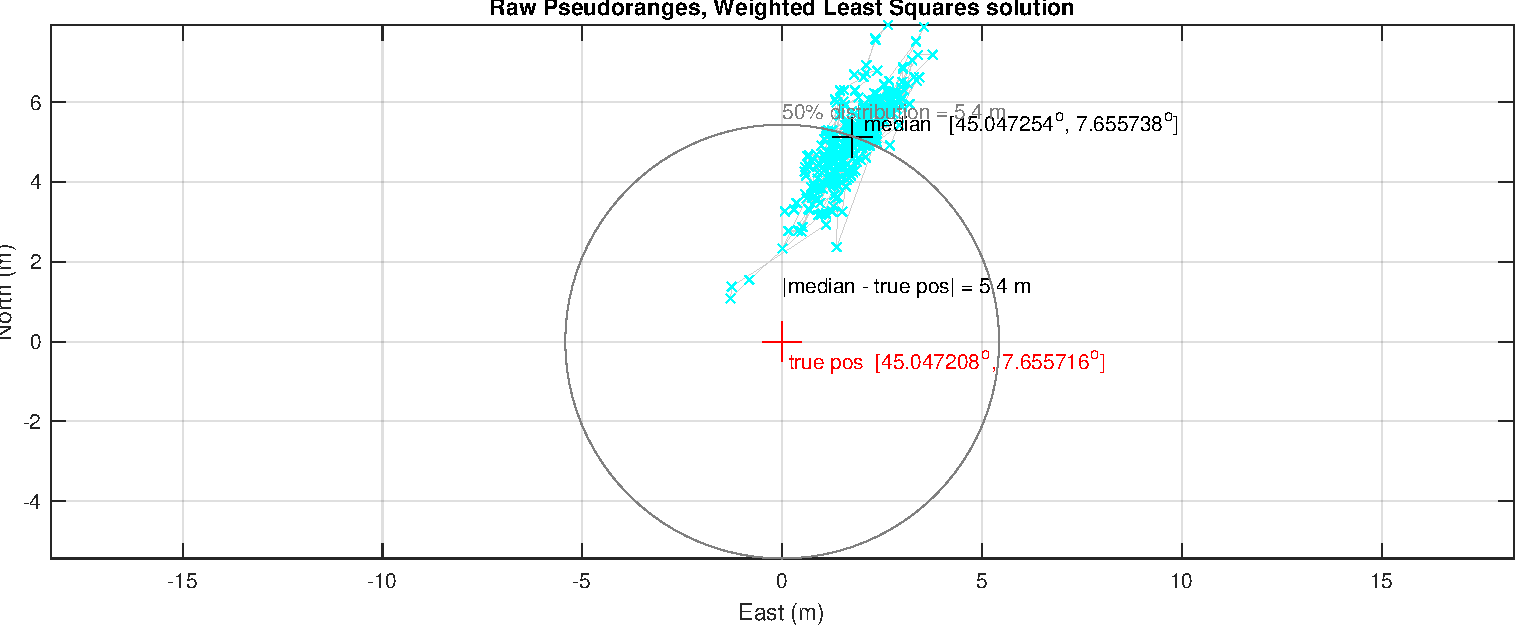
\includegraphics[width=1.00\linewidth]{images/pos_punto_3.pdf}
        \caption{Positioning geoplot for logs collected in open-sky conditions, correlated with true position (\ref{sec:opensky})}
        \label{fig:pos_punto_3}

    \end{minipage}
\end{figure}

\begin{figure}[H]
    \centering
    \begin{minipage}[b]{0.48\linewidth}
        \centering
        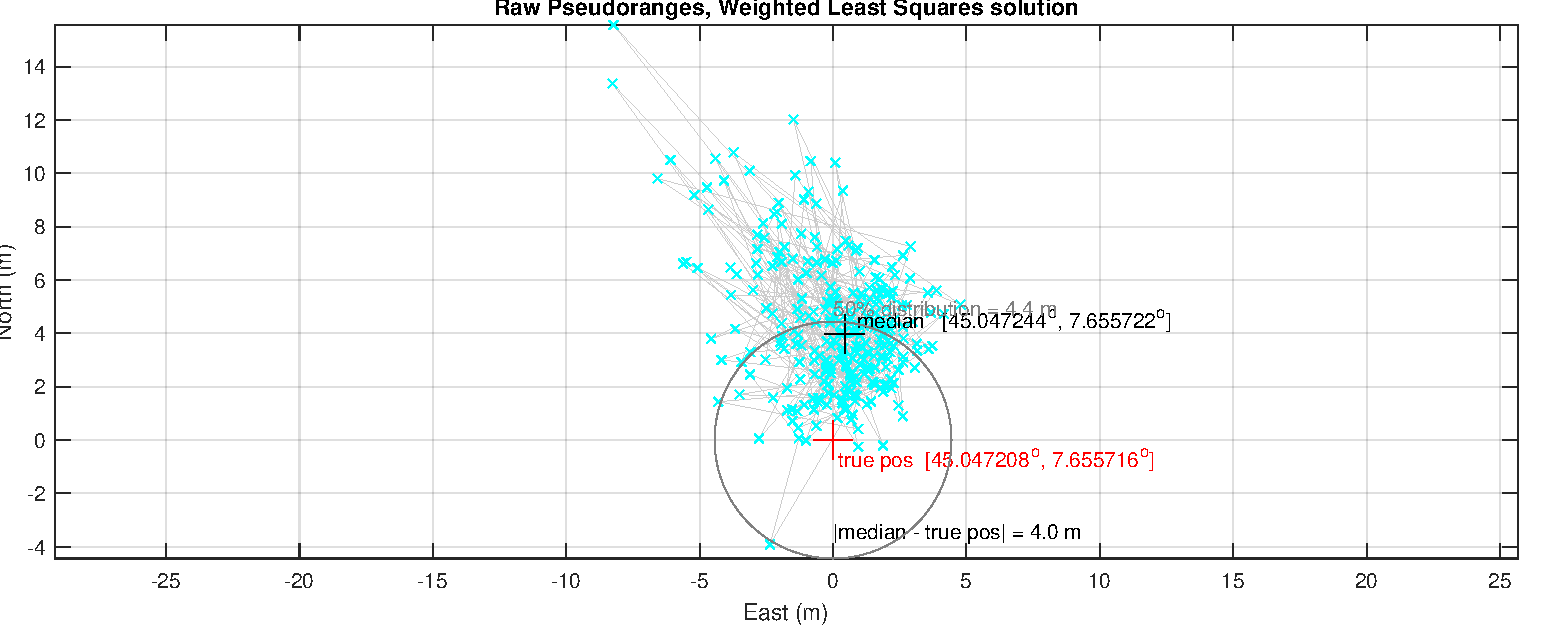
\includegraphics[width=1.00\linewidth]{images/carne_pos.pdf}
        \captionsetup{labelformat=empty}
        \caption{\textbf{Figure \ref{fig:carne_pos}:} Positioning geoplot for logs collected in the interference scenario (\ref{sec:opensky})}
        \end{minipage}
    \hfill
    \begin{minipage}[b]{0.48\linewidth}
        \centering
        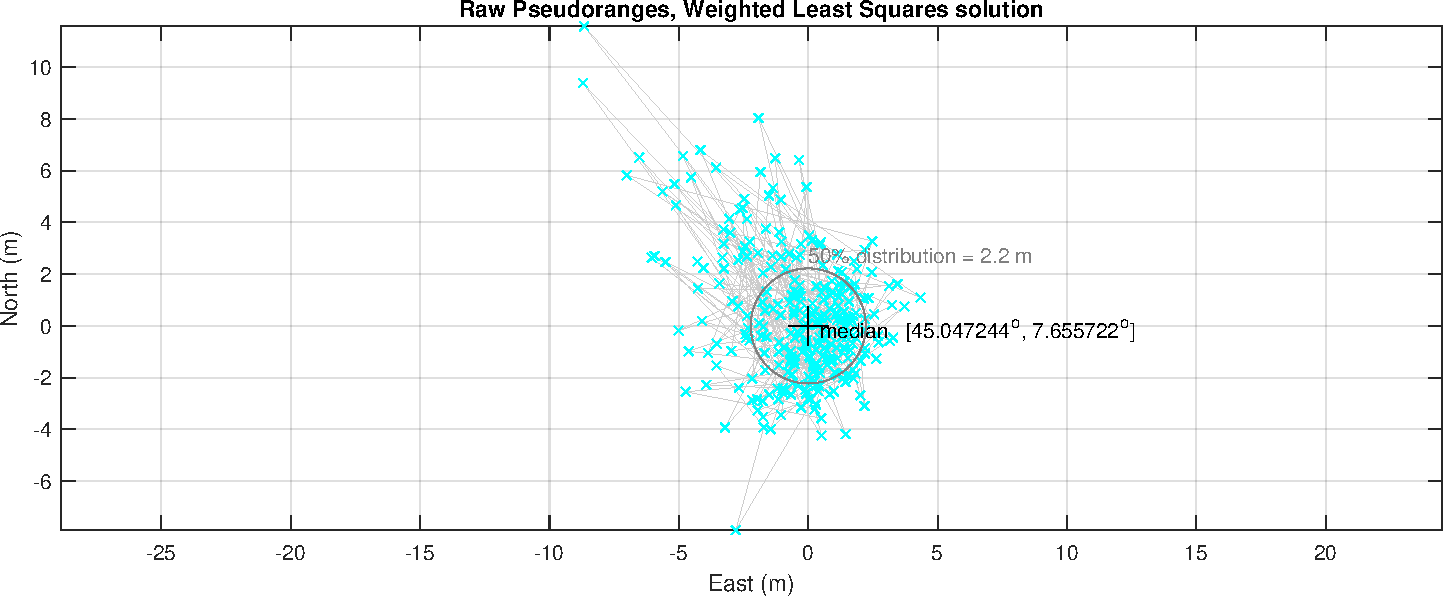
\includegraphics[width=1.00\linewidth]{images/carne_pos_precision.pdf}
        \caption{Positioning geoplot for logs collected in the interference scenario, correlated with true position (\ref{sec:opensky})}
        \label{fig:carne_pos_precision}

    \end{minipage}
\end{figure}


\begin{figure}[H]
    \centering
    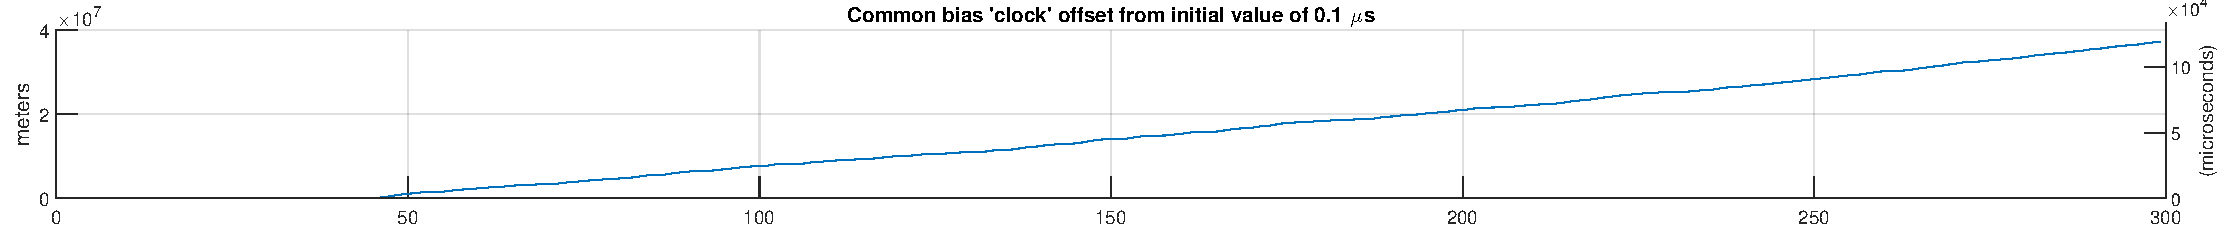
\includegraphics[width=0.95\linewidth]{images/discontinuity_bias_clock.pdf}
    \caption{Common bias clock offset in HW clock discontinuity} 
    \label{fig:discontinuity_bias_clock}
\end{figure}

\begin{figure}[H]
        \centering
        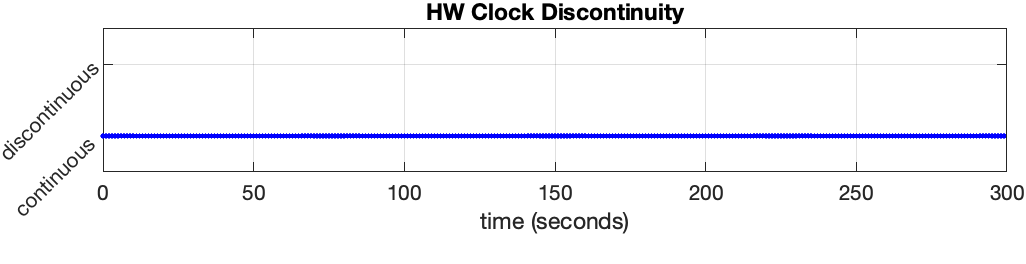
\includegraphics[width=0.85\linewidth]{images/continuity_gnss_log.png}
        \caption{Status of the GNSS hardware clock over time with GNSSLogger and GPSTest in parallel}
        \label{fig:GNSSLogger-continuity}
\end{figure}

\begin{figure}[H]
    \centering
    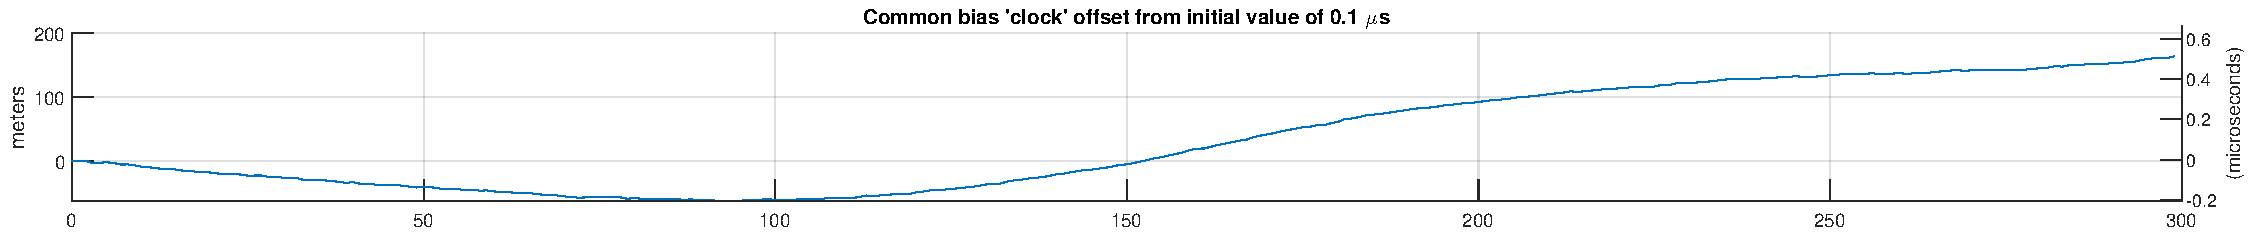
\includegraphics[width=0.95\linewidth]{images/continuity_bias_clock.pdf}
    \caption{Common bias clock offset in open-sky and HW clock continuity conditions (\ref{sec:opensky})} 
    \label{fig:continuity_bias_clock}
\end{figure}


\begin{figure}[H]
    \centering
    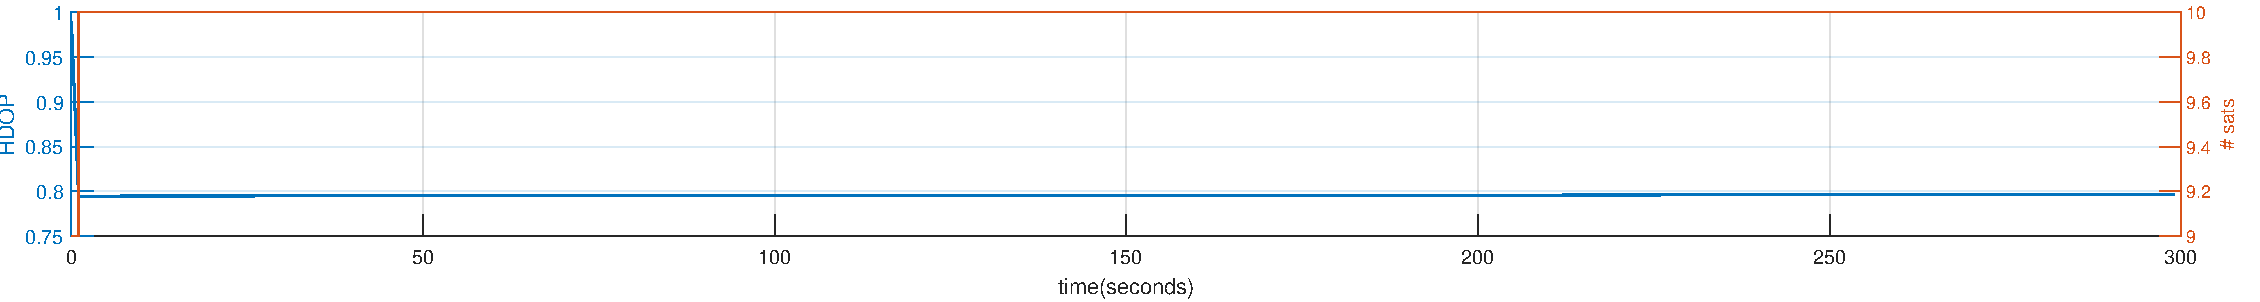
\includegraphics[width=1.00
    \linewidth]{images/hdop_punto_3.pdf}
    \caption{Horizontal diluition and number of satellites for logs collected in open-sky conditions (\ref{sec:opensky})}
    \label{fig:hdop_punto_3}
\end{figure}

\begin{figure}[H]
    \centering
    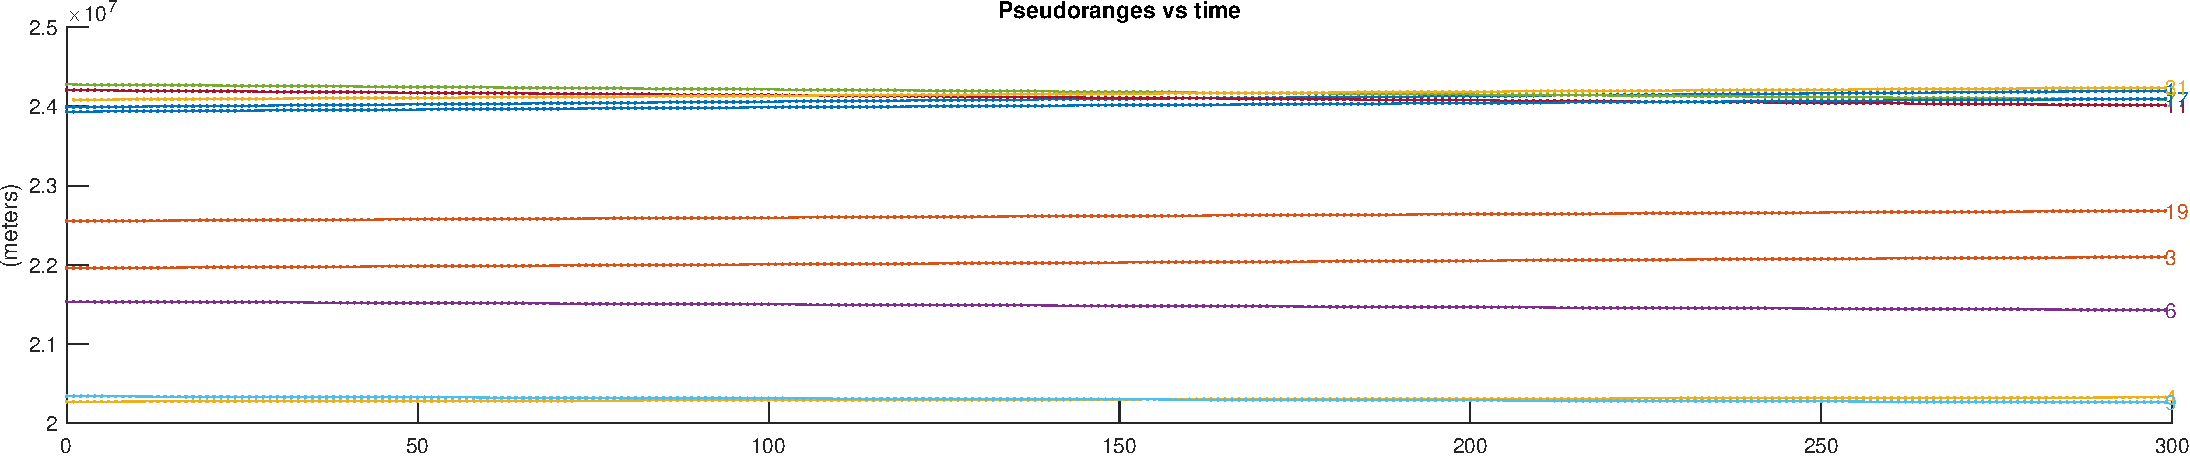
\includegraphics[width=1.00
    \linewidth]{images/punto3_pseudoranges.pdf}
    \caption{Pseudoranges vs. time for logs collected in open-sky conditions (\ref{sec:opensky})}
    \label{fig:pseudoranges_opensky}
\end{figure}

\begin{figure}[H]
    \centering
    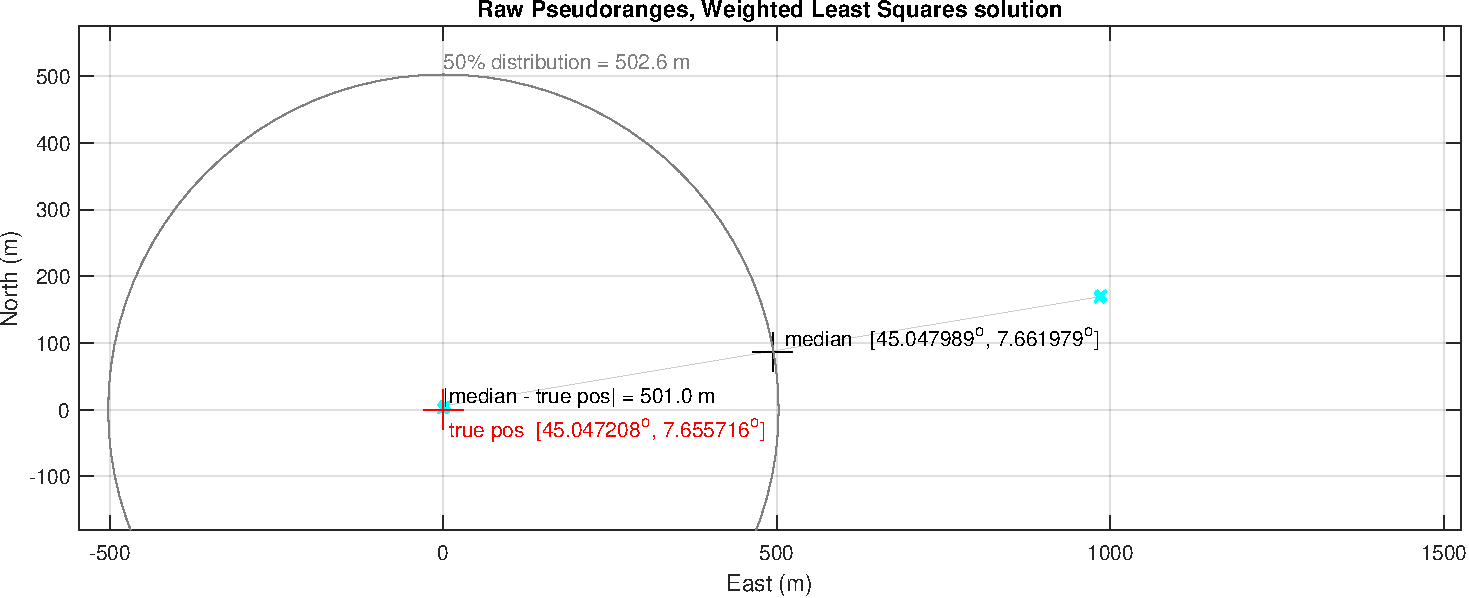
\includegraphics[width=1.00
    \linewidth]{images/pos_spoofed_no_delay.pdf}
    \caption{Positioning geoplot after applying spoofing to a location 1 Km from the real one, with no additional time delay used}
    \label{fig:pos_spoofed_no_delay}
\end{figure}

\begin{figure}[H]
    \centering
    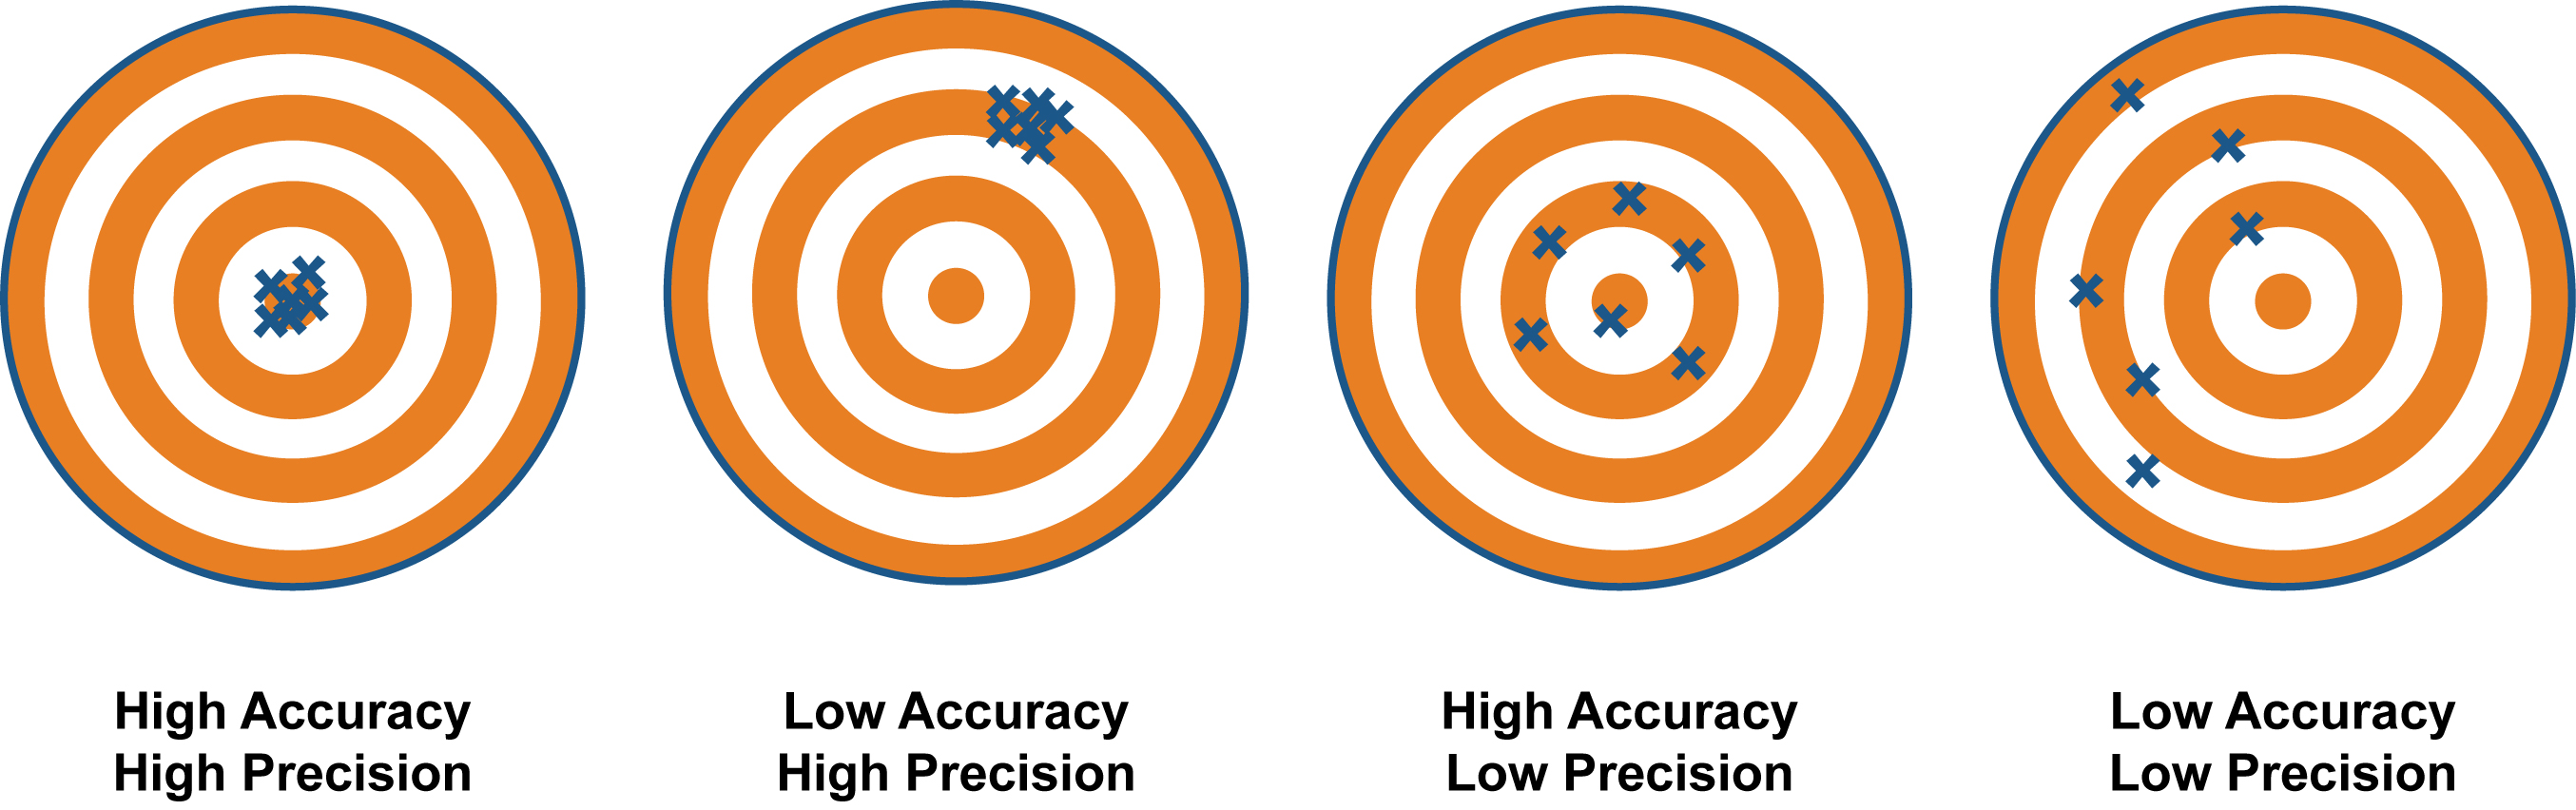
\includegraphics[width=0.50
    \linewidth]{images/Accuracy-vs-precision1.jpg}
    \caption{Accuracy vs. Precision}
    \label{fig:accPos}
\end{figure}

% \section{Appendix section title}
% \label{sec:underwater-comm}
% \colorbox{yellow}{Do we need this?}

% \begin{minted}[fontsize=\small, breaklines]{python}
% import subprocess
% import time
% import numpy as np
% import csv

% def run_iperf(name, server_ip, bind_ip, reverse, repetitions, pcap_fileNoExt, server_port, duration, udp, bitrate, app_buff_length):
% \end{minted}


\end{document}


%%% Local Variables:
%%% mode: latex
%%% TeX-master: t
%%% End:
